\documentclass[11pt]{article}

\usepackage{amsmath,stackrel}
\usepackage{amssymb}% http://ctan.org/pkg/amssymb

\usepackage[margin=1.05in]{geometry}
\usepackage{tikz}
\usetikzlibrary{arrows}
\usetikzlibrary{decorations.pathreplacing}
%\usepgflibrary{patterns}
\usetikzlibrary{patterns}

\usepackage{adjustbox}
\usepackage{listings}

\usepackage{color}
\definecolor{secblue}{HTML}{3B5E7F}
\definecolor{mycolor1}{RGB}{184,183,255}
\definecolor{mycolor2}{RGB}{255,  1,208}
\definecolor{mycolor3}{RGB}{  1,255,  2}
\definecolor{mypink}{rgb}{0.98,0.85,0.87}
%\definecolor{mypink}{rgb}{0.98,0.75,0.987}
\definecolor{listinggray}{gray}{0.9}
\definecolor{lbcolor}{rgb}{0.9,0.9,0.9}

\def\yy{\\\rowcolor{red}}
\usepackage{colortbl,ifthen}
\newcounter{line}
\newcommand\xx{%
  \addtocounter{line}{1}%
  \ifthenelse{\isodd{\value{line}}}{\\\rowcolor{listinggray}}{\\}}


\usepackage{algorithm}
\usepackage{algpseudocode}
\usepackage{comment}
\usepackage{xspace}
\usepackage{hyperref}

\usepackage{longtable}


\lstset{
backgroundcolor=\color{lbcolor},
    tabsize=4,    
%   rulecolor=,
    language=[GNU]C++,
        basicstyle=\scriptsize,
        upquote=true,
        aboveskip={1.5\baselineskip},
        columns=fixed,
        showstringspaces=false,
        extendedchars=false,
        breaklines=true,
        prebreak = \raisebox{0ex}[0ex][0ex]{\ensuremath{\hookleftarrow}},
        frame=single,
        numbers=left,
        showtabs=false,
        showspaces=false,
        showstringspaces=false,
        identifierstyle=\ttfamily,
        keywordstyle=\color[rgb]{0,0,1},
        commentstyle=\color[rgb]{0.026,0.112,0.095},
        stringstyle=\color[rgb]{0.627,0.126,0.941},
        numberstyle=\color[rgb]{0.205, 0.142, 0.73},
%        \lstdefinestyle{C++}{language=C++,style=numbers}’.
}
\lstset{
    backgroundcolor=\color{lbcolor},
    tabsize=4,
  language=C++,
  captionpos=b,
  tabsize=3,
  frame=lines,
  numbers=left,
  numberstyle=\tiny,
  numbersep=5pt,
  breaklines=true,
  showstringspaces=false,
  basicstyle=\footnotesize,
%  identifierstyle=\color{magenta},
  keywordstyle=\color[rgb]{0,0,1},
  commentstyle=\color[rgb]{0,0.45,0},
  stringstyle=\color{red}
  }

%\usepackage[utf8]{inputenc}
%\usepackage[x11names,svgnames]{xcolor}
\usepackage{graphicx}
\usepackage{fourier-orns}
%\usepackage[framemethod=tikz]{mdframed}
%\usetikzlibrary{calc}

\makeatletter
% Default settings for warnings
    \newcommand{\warningSymbol}{\raisebox{0.9\depth}{\danger}}

    \definecolor{warningColorText}{named}{blue}
    %\definecolor{warningColorLine}{named}{Red3}
    %\definecolor{warningColorBack}{named}{LemonChiffon1}
    %\definecolor{warningColorBackSymbol}{named}{white}

% Inline mode
    \newcommand{\warningcp}[1]{%
        \smallskip \noindent \textcolor{warningColorText}{\warningSymbol{}}\,\textbf{#1} %
    }

    %\newmdenv[style=warning]{@Warning}
    \newenvironment{Warning}{\let\warningcp\relax\begin{@Warning}}{\end{@Warning}}
\makeatother



\algnewcommand\algorithmicinput{\textbf{Input:}}
\algnewcommand\Input{\item[\algorithmicinput]}
\algnewcommand\algorithmicinit{\textbf{Initialization:}}
\algnewcommand\Init{\item[\algorithmicinit]}
\algnewcommand\algorithmicoutput{\textbf{Output:}}
\algnewcommand\Output{\item[\algorithmicoutput]}

\newcommand{\Hi}{\texttt{HiOp}\xspace}

\begin{document}
%\title{}

\begin{titlepage}



\begin{center}
\ 
\vspace{3cm}

  {\huge\bfseries \Hi\ -- User Guide} \\[14pt]
  {\large\bfseries version 0.6}

\vspace{3cm}

{\large\emph{by}}

\vspace{1.25cm}

 {\Large\bfseries Cosmin G. Petra}, {\Large\bfseries Nai-Yuan Chiang}, and {\Large\bfseries Jingyi Wang}
 
\vspace{1.1cm}

{\bfseries\Large{\textcolor{blue}{Center for Applied Scientific Computing\\
Lawrence Livermore National Laboratory}}}\\[10pt]


{\Large{7000 East Avenue, \\Livermore, CA 94550, USA.}}


\vspace{4.75cm}

 \textcolor{violet}{{\large\bfseries Oct 15, 2017} \\
{\large\bfseries Updated  March 31, 2022}}

\vspace{0.75cm}

{\Large\bfseries \textcolor{violet}{Technical report LLNL-SM-743591}}




%\maketitle

\end{center}
\end{titlepage}

\newpage

 \ 
 
\bigskip

\bigskip

%\fbox{

%\section*{Disclaimer and acknowledgments}

\noindent\fcolorbox{black}{mypink}{\begin{minipage}{0.98\textwidth} \bfseries 
This document was prepared as an account of work sponsored by an agency of the United States government.
Neither the United States government nor Lawrence Livermore National Security, LLC, nor any of their employees
makes any warranty, expressed or implied, or assumes any legal liability or responsibility for the accuracy,
completeness, or usefulness of any information, apparatus, product, or process disclosed, or represents that its use
would not infringe privately owned rights. Reference herein to any specific commercial product, process, or service
by trade name, trademark, manufacturer, or otherwise does not necessarily constitute or imply its endorsement,
recommendation, or favoring by the United States government or Lawrence Livermore National Security, LLC. The
views and opinions of authors expressed herein do not necessarily state or reflect those of the United States
government or Lawrence Livermore National Security, LLC, and shall not be used for advertising or product
endorsement purposes.
\end{minipage}}

\bigskip

\bigskip

\bigskip

\bigskip

\bigskip

\bigskip

\bigskip

\bigskip

\noindent\fcolorbox{black}{mypink}{\begin{minipage}{0.98\textwidth} \bfseries 
This work performed under the auspices of the U.S. Department of Energy by Lawrence Livermore National Laboratory under Contract DE-AC52-07NA27344. 
\end{minipage}}

\bigskip

\bigskip


%\noindent\fcolorbox{black}{lightgray}{\begin{minipage}{0.95\textwidth}
%The author also acknowledges the support from the LDRD Program of Lawrence Livermore National Laboratory under the projects 16-ERD-025 and 17-SI-005 and from the Department of Energy's Office of Science through the Advanced Scientific Computing Research (ASCR) program.
%\end{minipage}}


\newpage

\tableofcontents

\newpage

\section{Introduction}

This document describes the \Hi suite of HPC optimization solvers for some large-scale nonconvex nonlinear programming problems (NLPs). Two main classes of optimization problems are supported. First class consists of NLPs with extremely large number of variables  but with a relatively small number of general constraints; the solver for these problems is a  memory-distributed, MPI-based quasi-Newton interior-point solver using limited-memory approximations for the Hessians. The second class of problems consists of NLPs that have dense and sparse blocks, for which a ``Newton'' interior-point solver is available toghether with a specialized, so called mixed dense-sparse (MDS) linear algebra capable of achieving good performance on host-device, \textit{i.e.}, CPU-GPU, computing hardware. 

This document includes instructions on how to obtain and
build \Hi and a description of its interface, user options, and use as an optimization library. Guidelines on how is best to use the solver for parallel computations are also provided. The document generally targets users of \Hi, but also contains information relevant to potential developers or advanced users; these are strongly encouraged to also read the paper on the computational approach implemented in \Hi~\cite{petra_hiop}.


While the MPI quasi-Newton solver of \texttt{Hiop} targets DAE- and PDE-constrained optimization problems formulated in a ``reduced-space'' approach, it can be used for general nonconvex nonlinear optimization as well. For efficiency considerations, it is recommended to \textit{use quasi-Newton \texttt{Hiop} for NLPs that have a relatively small number of general constraints}, say less than $100$; note that there are no restrictions on the number of bounds constraints, \textit{e.g.}, one can specify simple bounds on any, and potentially all the decision variables without affecting the computational efficiency. The minimizers computed by \Hi satisfies \textit{local} first-order optimality conditions.

The goal of quasi-Newton solver of \Hi is to remove the parallelization limitations of existing state-of-the-art solvers for nonlinear programming (NLP) and match/surpass the parallel scalability of the underlying PDE or DAE solver. Such limitation occurs whenever the dimensionality of the optimization space  is as large as the dimensionality of the discretization of the differential systems of equations governing the optimization. In these cases, the use of existing NLP solvers  results in i. considerable long time spent in optimization, which affects the parallel scalability, and/or ii. memory requirements beyond the memory capacity of the computational node that runs the optimization. \Hi removes these scalability/parallelization bottlenecks (for certain optimization problems described above) by offering interface for a \textit{memory-distributed} specification of the problem and parallelizing the optimization search using specialized parallel linear algebra technique.

The general computational approach in \Hi is to use existing state-of-the-art NLP algorithms and develop linear algebra kernels tailored to the specific of this
class of problems. \Hi is based on an interior-point line search filter method~\cite{waecther_05_ipopt2,waecther_05_ipopt} and follows the implementation details from~\cite{waecther_05_ipopt0}, which is the implementation paper for IPOPT open-source NLP solver. The quasi-Newton approach is based on limited-memory secant approximations of the Hessian~\cite{ByrdNocedalSchnabel_94_quasiNewtonRepres}, which is generalized as required by the specific of interior-point methods for constrained optimization problems~\cite{petra_hiop}. The specialized linear algebra decomposition is obtained by using a Schur-complement reduction that
leverages the fact that the quasi-Newton Hessian matrix has a small number of
dense blocks that border a low-rank update of a diagonal matrix. The technique is described  in ~\cite{petra_hiop}. The Newton interior-point solver of \Hi uses linear algebra specialized to the particular form of the MDS NLPs supported by this solver, for more details consult Section~\ref{sec:mds}. 

The C++ parallel implementation in \Hi
is  lightweight and portable since it is expressed and implemented  only in terms of parallel (multi-)vector operations (implemented internally using BLAS level 1 and level 2 operations and MPI for communication) and BLAS level 3 and LAPACK operations for small dense matrices.

By using multithreadead BLAS and LAPACK libraries, \textit{e.g.}, INTEL MKL, GotoBlas, Atlas, etc, additional,  intra-node parallelism can be achieved. These libraries are usually  machine/hardware specific and available for a variety of computer architectures. A list of BLAS/LAPACK implementations can be found at 
%\begin{lstlisting} 
\url{https://en.wikipedia.org/wiki/Basic_Linear_Algebra_Subprograms\#Implementations}. 
%\end{lstlisting}
%The salient idea

\section{Installing/building \Hi}
\Hi is available on  Lawrence Livermore National Laboratory (LLNL)  github's page at 
\url{https://github.com/LLNL/hiop}. \Hi can be obtained by cloning the repository or by downloading the release archive(s). To clone from the repository, one needs to simply run
\begin{verbatim}
> git clone https://github.com/LLNL/hiop.git
\end{verbatim}

\subsection{Prerequisites} 
\Hi is written in C++11. At minimum, \Hi  requires BLAS and LAPACK, however, the more advanced solvers require additional dependencies (MPI, RAJA and Umpire, CUDA, MAGMA, CoinHSL, PARDISO, STRUMPACK, etc.). The CMake-based build system of \Hi generally detects these prerequisites automatically and warns the user when such prerequisites are missing.

At this point the build system only supports macOS and Linux operating systems. On the other hand, other than the build system, \Hi's code is  platform independent and should run fine on Windows as well.


\subsection{Building, testing, and installing \Hi}
The build system is based on CMake. Up-to-date detailed information about \Hi custom builds and installs are kept at \url{https://github.com/LLNL/hiop}. 

A quick way to build and code is run the following commands in the `build\//' directory in the root \Hi directory: 
\begin{verbatim}
> cmake ..
> make all
> make test
> make install
\end{verbatim}
This will compile, build the static library and example executables, perform a couple of tests to detect potential issues during the installation, and will install \Hi's header and the static library in the root directory under `\_build\_defaultDist\//'

\subsection{Support of host-device computations using (generic)CPU-(NVIDIA)GPU hardware}

Starting version 0.3, \Hi offers support for offloading computations to NVIDIA GPU accelerators when solving NLPs in the mixed dense-sparse (MDS) form. Support for GPUs should be enabled during the build by using \texttt{-DHIOP\_USE\_GPU} option with \texttt{cmake}, which will result in using the GPU accelerators for the internal linear solves; in addition, the options \texttt{-DHIOP\_USE\_RAJA} will employ RAJA portability abstraction to perform the remaining linear algebra computations on the GPU device or on the host (with OpenMP acceleration). When RAJA is enabled, \Hi can be instructed to use Umpire as memory manager (see option \texttt{mem\_space}). As of v0.5, the combination of RAJA and Umpire enables \Hi to perform iterations of the Newton IPM solver solely on the device by setting option \texttt{mem\_space} to \texttt{device} and option \texttt{compute\_mode} to \texttt{gpu}. 

\Hi's \texttt{cmake} build system is quite versatile to find the dependencies required to offload computations to the device GPUs since was developed and tested on a few GPU-enabled HPC platforms at Oak Ridge, Lawrence Livermore, and Pacific Northwest National Laboratories. These dependencies consist of CUDA library version 10.1 or later and a recent Magma linear solver library (as well as a physical NVIDIA GPU device). \Hi offers an extensive build support for using customized NVIDIA libraries and/or Magma solver as well as for advanced troubleshooting. The user is referred to \texttt{cmake/FindHiopCudaLibraries.cmake} and \texttt{cmake/FindMagma.cmake} scripts.

\warningcp{Note: } Installing NVIDIA CUDA (and likely the NVIDIA driver) and/or building Magma can be quite challenging. The user is encouraged to rely on preinstalled versions of these, as they are available via \texttt{module} utility on virtually all high-performance computing machines. An example of how to satisfy all the GPU dependencies on Summit supercomputer at Oak Ridge National Lab with a one commands are available at \url{https://github.com/LLNL/hiop/blob/master/README_summit.md}.

\subsection{Building extra features}

To build the documentation for \Hi, enable the 
\texttt{HIOP\_BUILD\_DOCUMENTATION} option when configuring. This option can 
only be enabled if a \texttt{doxygen} executable is available in the path. This 
option adds the \texttt{make} targets \texttt{doc} and \texttt{install\_doc} 
which build and install the documentation respectively. When installed, 
\texttt{html} and \LaTeX{}/pdf documentation may be found under 
\texttt{<install prefix>/doc/html} and \texttt{<install prefix>/doc/html}, 
respectively.

To build every configuration of HiOp for testing purposes, the build script has an option \texttt{./BUILD.sh --full-build-matrix}. See the testing section of \texttt{README\_developers.md} for more information.

Additional \Hi features not yet mentioned may be found in the top of the top-level \texttt{CMakeLists.txt} file with a brief description.

\section{Interfacing with \Hi}
Once \Hi is built, it can be used as the optimization solver in your application through the \Hi's C++ interfaces and by linking with the static library. A shared dynamic load library can be also built using \texttt{HIOP\_BUILD\_SHARED} option with cmake. There are three types of nonlinear optimization or NLP formulations currently supported by \Hi. They are described and discussed by the subsequent sections.

\subsection{The NLP with \textit{dense} constraints formulation requiring \textit{up to first-order} derivative information}
A first class of problems supported by \Hi consists of nonlinear nonconvex NLP with \textit{dense} constraints of the form
\begin{align}
&&&&\min_{x\in\mathbb{R}^n} & \hspace{0.5cm} f(x) &&&& \label{obj}\\
&&&&\textnormal{s.t.} &\hspace{0.5cm}  c(x)=c_E &[y_c]&&&\\
&&[v_l]&&& \hspace{0.5cm} d_l \leq d(x) \leq d_u  &[v_u]&&&\label{ineq} \\
&&[z_u]&&& \hspace{0.5cm} x_l \leq x \leq x_u & [z_u] &&&\label{bounds}
\end{align}
Here $f:\mathbb{R}^n\rightarrow\mathbb{R}$, $c:\mathbb{R}^n\rightarrow\mathbb{R}^{m_E}$, $d:\mathbb{R}^n\rightarrow\mathbb{R}^{m_I}$. The bounds appearing in the inequality constraints~\eqref{ineq} are assumed to be $d^l\in\mathbb{R}^{m_I}\cup\{-\infty\}$, $d^u\in\mathbb{R}^{m_I}\cup\{+\infty\}$, $d_i^l < d_i^u$, and at least of one of $d_i^l$ and $d_i^u$ are finite for all $i\in\{1,\ldots,m_I\}$. The bounds in~\eqref{bounds} are such that $x^l\in\mathbb{R}^{n}\cup\{-\infty\}$, $x^u\in\mathbb{R}^{n}\cup\{+\infty\}$, and $x_i^l < x_i^u$, $i\in\{1,\ldots,n\}$. The quantities insides brackets are the Lagrange multipliers of the constraints. Whenever a bound is infinite, the corresponding multiplier is by convention zero.

The following quantities are required by \Hi:
\begin{itemize}
\item[D1] objective and constraint functions $f(x)$, $c(x)$, $d(x)$;
\item[D2] the first-order derivatives of the above: $\nabla f(x)$, $Jc(x)$, $Jd(x)$;
\item[D3] the simple bounds $x_l$ and $x_u$, the inequalities bounds: $d_l$ and $d_u$, and the right-hand size of the equality constraints $c_E$.
\end{itemize}

\subsubsection{The C++ interface}
The above optimization problem~\eqref{obj}-\eqref{bounds} can be specified by using the C++ interface, namely by deriving and providing an implementation for the \texttt{hiop::hiopInterfaceDenseConstraints} abstract class.

 We present next the methods of this abstract class that needs to be implemented in order to specify the parts D1-D3 of the optimization problem. 

 \warningcp{Note:} All the functions that return \texttt{bool} should return \texttt{false} when an error occurs, otherwise should return \texttt{true}.

 \warningcp{Note:} The C++ interface uses the integer types \texttt{size\_type} and \texttt{index\_type}.  The type \texttt{hiop::size\_type} is used for container (\textit{e.g.,} NLPs, vectors, matrices, etc.) sizes and generally holds a nonnegative integer. The \texttt{hiop::index\_type} type should be used for indexes within containers and is generally holding a nonnegative integer. These two types are defined within \Hi namespace (see \texttt{hiop\_defs.h}) and currently set to \texttt{int}. This choice allows a streamlined integration (that is, type conversions are not needed and arrays of indexes can be reused) with the low level linear algebra libraries, such as sparse and dense linear solver libraries, which generally use \texttt{int}.

\subsubsection{Specifying the optimization problem}

All the methods of this section are ``pure'' virtual in \texttt{hiop::hiopInterfaceDenseConstraints} abstract class  and need to be provided by the user implementation.

\begin{lstlisting} 
bool get_prob_sizes(size_type& n, size_type& m);
\end{lstlisting} 
\noindent Provides the number of decision variables and the number of constraints ($m=m_E+m_I$).


\begin{lstlisting} 
bool get_vars_info(const size_type& n, double *xlow, double* xupp, 
                   NonlinearityType* type);
\end{lstlisting} 

\noindent Provides the lower and upper bounds $x_l$ and $x_u$ on the decision variables. When a variable (let us say the $i^{th}$) has no lower or/and upper bounds, the  $i^{th}$ entry of xlow and/or xupp should be less than $-1^{20}$ or/and larger than $1^{20}$, respectively. The last argument is not used and can set to any value of the enum \texttt{hiop::hiopInterfaceDenseConstraints::NonlinearityType}.

\begin{lstlisting} 
bool get_cons_info(const size_type& m, double* clow, double* cupp, 
                   NonlinearityType* type);
\end{lstlisting}
\noindent Similar to the above, but for the inequality bounds $d_l$ and $d_u$. For equalities, set the corresponding entries in clow and cupp equal to the desired value (from $c_E$).


\begin{lstlisting} 
bool eval_f(const size_type& n, 
            const double* x, bool new_x, 
            double& obj_value);
\end{lstlisting} 

\noindent Implement this method to compute the function value $f(x)$ in \texttt{obj\_value} for the provided decision variables $x$. The input argument \texttt{new\_x} specifies whether the variables $x$ have been changed since the previous call of one of the \texttt{eval\_} methods. Use this argument to ``buffer'' the objective and gradients function and derivative evaluations when this is possible.

\begin{lstlisting} 
bool eval_grad_f(const size_type& n, 
                 const double* x, bool new_x, 
                 double* gradf);
\end{lstlisting} 

\noindent Same as above but for $\nabla f(x)$.

\begin{lstlisting} 
 bool eval_cons(const size_type& n, const size_type& m, 
                const size_type& num_cons,
				    const index_type* idx_cons, const double* x, 
			       bool new_x, double* cons);
\end{lstlisting} 

\noindent Implement this method to provide the value of the constraints $c(x)$ and/or $d(x)$. The input parameter \texttt{num\_cons} specifies how many constraints (out of \texttt{m}) needs to evaluated; \texttt{idx\_cons} array specifies the indexes, which are zero-based, of the constraints  and is of size \texttt{num\_cons}. These values should be provided in \texttt{cons}, which is also an array of size \texttt{num\_cons}.

\begin{lstlisting} 
bool 
eval_Jac_cons(const size_type& n, const size_type& m, 
			     const size_type& num_cons, const index_type* idx_cons,  
			     const double* x, bool new_x,
			     double* Jac);
\end{lstlisting} 

\noindent Implement this method to provide the Jacobian of a subset of the  constraints $c(x)$ and/or $d(x)$ in \texttt{Jac}; as for \texttt{eval\_cons}, this subset is specified by the array of row indexes \texttt{idx\_cons}. The array \texttt{Jac} should contain the Jacobian row-wise, meaning that the each row of the Jacobian is contiguous in memory and starts right after the previous row.


\subsubsection{Specifying the inter-process/memory distribution of the   problem}

\Hi uses \textit{data parallelism}, meaning that the data [D1]-[D3] of the optimization problem is distributed across processes (MPI ranks). It is \textbf{crucial} to understand the data distribution scheme in order to use \Hi's interface properly. 

The general rule of thumb is to distribute any data of the problem with storage depending on $n$, namely the decision variables $x$ and their bounds $x_l$ and $x_u$, the gradient $\nabla f(x)$, and the Jacobians $Jc(x)$ and $Jd(x)$. The Jacobians, which are assumed to be dense matrices with $n$ columns, are distributed column-wise.

\begin{figure}[h]
\centering
%\documentclass[11pt]{article}


%\begin{document}

%\section{Introduction}

\trimbox{0.5cm 0.cm 0cm 0cm} {
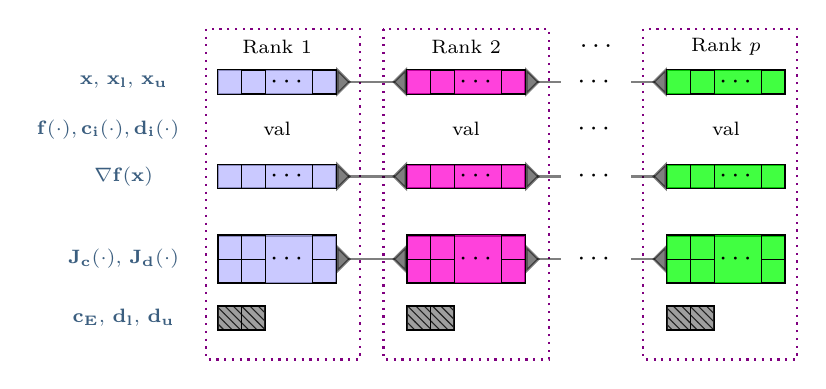
\begin{tikzpicture}[scale=.6]

%\node[inner sep=0pt] (cube) at (-7.5,-4)  {\includegraphics[width=.3\textwidth]{images/partition-2048-a}};

%\begin{scope}[every node/.append style={xslant=0.017,yslant=-0.04},xslant=0.017,yslant=-0.04]
%  %\shade[right color=gray!10, left color=black!50, semitransparent] (-10.5,-2.5) rectangle +(4,1);
%  \node[anchor=center] at (-8.,-3.75) {{\color{white} \textbf{Material and \ \ \ }}};
%  \node[anchor=center] at (-8.75,-4.35) {{\color{white} \textbf{design domain}}};
%\end{scope}

%\node[anchor=center,rotate=20,opaque=0.7] at (7.5,-4.75) {\large\color{subsecblue}\textbf{Optimization computational layout}};

%the table lines
\draw[thick,dotted,violet](2.25,0.375) rectangle+(3.25,-7.);
\draw[thick,dotted,violet](6.,0.375) rectangle+(3.5,-7.);
\draw[thick,dotted,violet](11.5,0.375) rectangle+(3.25,-7.); 

% line with procs
\draw[thick](3.75,0) node(proc1)[anchor=center]{\scriptsize Rank $1$};
\draw[thick](7.75,0) node(proc2){\scriptsize Rank $2$};
\draw[thick](10.5,0) node{$\ldots$ };
\draw[thick](13.25,0) node(procp){\scriptsize Rank $p$};


%arrowsfrom 3d-domain to procs

%\node(n1) at (-10.75,-1){};
%\node(n2) at (-7.75,-1){};
%\node(n3) at (-3.95,-5.15){};
%\path[every node/.style={font=\sffamily\small},semitransparent,gray]
%    (n1) edge[bend left,dashed,->,>=triangle 60,out=20, in=155] node [right] {} (proc1)
%    (n2) edge[bend left,dashed,->,>=triangle 60,out=20, in=155] node [right] {} (proc2)
%		(n3) edge[bend left,dashed,->,>=triangle 60,out=60, in=150] (procp);


%\draw[thick](n1) -- (proc1);

%Decision variable
%!\draw(1.,-0.75) node[anchor=center]{\color{secblue}{\textbf{\scriptsize Decision $\textbf{x}$}}};
\draw(0.5,-0.75) node[anchor=center]{\color{secblue}{\scriptsize $\mathbf{x}$, $\mathbf{x_l}$, $\mathbf{x_u}$ }};
\draw[thick](2.5,-1) rectangle+(2.5,0.5); \fill[mycolor1,fill opacity=0.75](2.5,-1) rectangle+(2.5,0.5); 
\draw(3.0,-1) rectangle +(.5,0.5);
\draw[thick](4.0,-0.75) node[anchor=center]{$\cdots$}; 
\draw(4.5,-1) rectangle+(.5,0.5);
\draw [<->, >=triangle 90 reversed, line width=0.2ex,semitransparent](5.,-.75) -- ++(1.5,0);

\draw[thick](6.5,-1) rectangle+(2.5,0.5); \fill[mycolor2,fill opacity=0.75](6.5,-1) rectangle+(2.5,0.5); 
\draw(7.0,-1) rectangle +(.5,0.5);
\draw[thick](8.0,-0.75) node[anchor=center]{$\cdots$}; 
\draw(8.5,-1) rectangle+(.5,0.5);
\draw [<-, >=triangle 90 reversed, line width=0.2ex,semitransparent](9,-0.75) -- ++(0.75,0);

\draw[thick](10.5,-0.75) node[anchor=center]{$\cdots$};
\draw [->, >=triangle 90 reversed, line width=0.2ex,semitransparent](11.25,-0.75) -- ++(0.75,0);


\draw[thick](12,-1) rectangle+(2.5,0.5); \fill[mycolor3,fill opacity=0.75](12,-1) rectangle+(2.5,0.5); 
\draw(12.5,-1) rectangle +(.5,0.5);
\draw[thick](13.5,-0.75) node[anchor=center]{$\cdots$}; 
\draw(14,-1) rectangle+(.5,0.5);

%f(x)
%\draw(0.75,-1.65) node[anchor=center]{{\footnotesize Objective \&} };
%\draw(0.75,-1.85) node[anchor=center]{{\footnotesize constraints} };
%!\draw(0.95,-1.75) node[anchor=center]{\color{secblue}{\scriptsize $\mathbf{f(x), g_i(x)}$ } };
\draw(0.25,-1.75) node[anchor=center]{\color{secblue}{\scriptsize $\mathbf{f(\cdot), c_i(\cdot), d_i(\cdot)}$ } };


%\draw[decorate,decoration={brace,mirror, amplitude=7pt},xshift=0pt,yshift=0pt]
%(2.5,-1.125) -- (5.0,-1.125) node [black,midway,yshift=-12.5pt] 
%{\scriptsize $f(x)$};
\draw(3.75,-1.75) node[anchor=center] {\scriptsize val};
\draw(7.75,-1.75) node[anchor=center] {\scriptsize val};
\draw[thick](10.5,-1.75) node[anchor=center]{$\cdots$};
\draw(13.25,-1.75) node[anchor=center] {\scriptsize val};

%\draw[decorate,decoration={brace,mirror, amplitude=7pt},xshift=0pt,yshift=0pt]
%(6.5,-1.75) -- (9.0,-1.125) node [black,midway,yshift=-12.5pt] 
%%!{\scriptsize $f_2(x_2)$};
%{\scriptsize $f(x)$};
%
%\draw[thick](10.5,-1.75) node[anchor=center]{$\cdots$};%
%
%\draw[decorate,decoration={brace,mirror, amplitude=7pt},xshift=0pt,yshift=0pt]
%(12.00,-1.125) -- (14.5,-1.125) node [black,midway,yshift=-12.5pt] 
%%!{ \scriptsize $f_p(x_p)$};
%{ \scriptsize $f_p(z_p)$};





%gradients
%\draw(0.75,-2.63) node[anchor=center]{{\footnotesize Gradients}};
%\draw(0.75,-3.02) node[anchor=center]{{\footnotesize $\nabla f(x)$, $\nabla g_i(x)$}};
%!\draw(0.7,-2.75) node[anchor=center]{\color{secblue}{\scriptsize $\mathbf{\nabla f(x), \nabla g_i(x)}$}};
\draw(0.5,-2.75) node[anchor=center]{\color{secblue}{\scriptsize $\mathbf{\nabla f(x)}$}};

\draw[thick](2.5,-3.0) rectangle+(2.5,0.5); \fill[mycolor1,fill opacity=0.75](2.5,-3.0) rectangle+(2.5,0.5); 
\draw(3.0,-3) rectangle +(.5,0.5);
\draw[thick](4.0,-2.75) node[anchor=center]{$\cdots$}; 
\draw(4.5,-3) rectangle+(.5,0.5);
\draw [<->, >=triangle 90 reversed, line width=0.2ex,semitransparent](5.,-2.75) -- ++(1.5,0);

\draw[thick](6.5,-3) rectangle+(2.5,0.5);\fill[mycolor2,fill opacity=0.75](6.5,-3) rectangle+(2.5,0.5);
\draw(7.0,-3) rectangle +(.5,0.5);
\draw[thick](8.0,-2.75) node[anchor=center]{$\cdots$}; 
\draw(8.5,-3) rectangle+(.5,0.5);
\draw [<-, >=triangle 90 reversed, line width=0.2ex,semitransparent](9,-2.75) -- ++(0.75,0);

\draw[thick](10.5,-2.75) node[anchor=center]{$\cdots$};
\draw [->, >=triangle 90 reversed, line width=0.2ex,semitransparent](11.25,-2.75) -- ++(0.75,0);

\draw[thick](12,-3) rectangle+(2.5,0.5); \fill[mycolor3,fill opacity=0.75](12,-3) rectangle+(2.5,0.5); 
\draw(12.5,-3) rectangle +(.5,0.5);
\draw[thick](13.5,-2.75) node[anchor=center]{$\cdots$}; 
\draw(14,-3) rectangle+(.5,0.5);

%Jacobians
\draw(0.5,-4.5) node[anchor=center]{\color{secblue}{\scriptsize $\mathbf{J_c(\cdot)}$, $\mathbf{J_d(\cdot)}$}};

%U
\draw[thick](2.5,-4) rectangle+(2.5,-1); \fill[mycolor1,fill opacity=0.75](2.5,-4) rectangle+(2.5,-1); 
\draw(3.0,-4) rectangle+(0.5,-0.5); \draw(3.0,-4.5)rectangle+(0.5,-0.5);
\draw(2.5,-4) rectangle+(0.5,-0.5); \draw(2.5,-4.5)rectangle+(0.5,-0.5);
%\draw(2.5,-4) grid[step=0.5]+(1,-1);
\draw[thick](4.0,-4.5) node[anchor=center]{$\cdots$}; 
\draw(4.5,-4) rectangle+(0.5,-0.5);
\draw(4.5,-4.5)rectangle+(0.5,-0.5);
%\node at(1.4,-4.5) [right,fill=green,opacity=.0,text opacity=1] {\color{secblue}{\scriptsize $\mathbf{U}$}};
\draw [<->, >=triangle 90 reversed, line width=0.2ex,semitransparent](5.,-4.5) -- ++(1.5,0);

\draw[thick](6.5,-4) rectangle+(2.5,-1); \fill[mycolor2,fill opacity=0.75](6.5,-4) rectangle+(2.5,-1);
\draw(7.0,-4) rectangle+(0.5,-0.5); \draw(7.0,-4.5)rectangle+(0.5,-0.5);
\draw(6.5,-4) rectangle+(0.5,-0.5); \draw(6.5,-4.5)rectangle+(0.5,-0.5);
%\draw(6.5,-4) grid[step=0.5]+(1,-1);
\draw[thick](8.0,-4.5) node[anchor=center]{$\cdots$}; 
\draw(8.5,-4) rectangle+(0.5,-0.5);
\draw(8.5,-4.5)rectangle+(0.5,-0.5);
\draw [<-, >=triangle 90 reversed, line width=0.2ex,semitransparent](9,-4.5) -- ++(0.75,0);

\draw[thick](10.5,-4.5) node[anchor=center]{$\cdots$};
\draw [->, >=triangle 90 reversed, line width=0.2ex,semitransparent](11.25,-4.5) -- ++(0.75,0);

\draw[thick](12,-4) rectangle+(2.5,-1);  \fill[mycolor3,fill opacity=0.75](12,-4) rectangle+(2.5,-1); 
\draw(12.0,-4) rectangle+(0.5,-0.5); \draw(12.0,-4.5)rectangle+(0.5,-0.5);
\draw(12.5,-4) rectangle+(0.5,-0.5); \draw(12.5,-4.5)rectangle+(0.5,-0.5);
%\draw(12,-4) grid[step=0.5]+(1,-1);
\draw[thick](13.5,-4.5) node[anchor=center]{$\cdots$}; 
\draw(14,-4) rectangle+(0.5,-0.5);
\draw(14,-4.5)rectangle+(0.5,-0.5);

%V
\draw(0.5,-5.75) node[anchor=center] {\color{secblue}{\scriptsize $\mathbf{c_E}$, $\mathbf{d_l}$, $\mathbf{d_u}$ }};
\draw[thick,pattern=north west lines] (2.5,-5.5) rectangle++(1,-0.5); \fill[semitransparent,darkgray] (2.5,-5.5) rectangle++(1,-0.5);\draw (2.5,-5.5) grid[step=0.5]+(1,-.5);
\draw[thick,pattern=north west lines] (6.5,-5.5) rectangle++(1,-0.5); \fill[semitransparent,darkgray] (6.5,-5.5) rectangle++(1,-0.5);\draw (6.5,-5.5) grid[step=0.5]+(1,-0.5); 
\draw[thick,pattern=north west lines] (12,-5.5) rectangle++(1,-0.5); \fill[semitransparent,darkgray] (12,-5.5) rectangle++(1,-0.5);\draw (12,-5.5) grid[step=0.5]+(1,-0.5);

%B0
%\node at(1.0,-7.25) [right,fill=green,opacity=.0,text opacity=1] {\color{secblue}{ \scriptsize $\mathbf{B_0}$} };
%\draw[thick](2.5,-7.5) rectangle+(2.5,0.5); \fill[mycolor1,fill opacity=0.75](2.5,-7.5) rectangle+(2.5,0.5); 
%\draw(3.0,-7.5) rectangle +(.5,0.5);
%\draw[thick](4.0,-7.25) node[anchor=center]{$\cdots$}; 
%\draw(4.5,-7.5) rectangle+(.5,0.5);
%\draw [<->, >=triangle 90 reversed, line width=0.2ex,semitransparent](5.,-7.25) -- ++(1.5,0);

%\draw[thick](6.5,-7.5) rectangle+(2.5,0.5); \fill[mycolor2,fill opacity=0.75](6.5,-7.5) rectangle+(2.5,0.5);
%\draw(7.0,-7.5) rectangle +(.5,0.5);
%\draw[thick](8.0,-7.25) node[anchor=center]{$\cdots$}; 
%\draw(8.5,-7.5) rectangle+(.5,0.5);
%\draw [<-, >=triangle 90 reversed, line width=0.2ex,semitransparent](9,-7.25) -- ++(0.75,0);

%\draw[thick](10.5,-7.25) node[anchor=center]{$\cdots$};
%\draw [->, >=triangle 90 reversed, line width=0.2ex,semitransparent](11.25,-7.25) -- ++(0.75,0);

%\draw[thick](12,-7.5) rectangle+(2.5,0.5); \fill[mycolor3,fill opacity=0.75](12,-7.5) rectangle+(2.5,0.5); 
%\draw(12.5,-7.5) rectangle +(.5,0.5);
%\draw[thick](13.5,-7.25) node[anchor=center]{$\cdots$}; 
%\draw(14,-7.5) rectangle+(.5,0.5);

\end{tikzpicture}
}



%\end{document}

\caption{Depiction of the distribution of the data of the optimization problem ~\eqref{obj}-\eqref{bounds} across MPI ranks. The vectors and matrices with storage dependent on the number of optimization variables are distributed. Other data, \textit{i.e.}, scalar function values or vectors of small size (shown in dashed dark grey boxes), are replicated on each rank.}
\label{diagr_distrib}
\end{figure}
%%\documentclass[11pt]{article}


%\begin{document}

%\section{Introduction}

\trimbox{0.5cm 0.cm 0cm 0cm} {
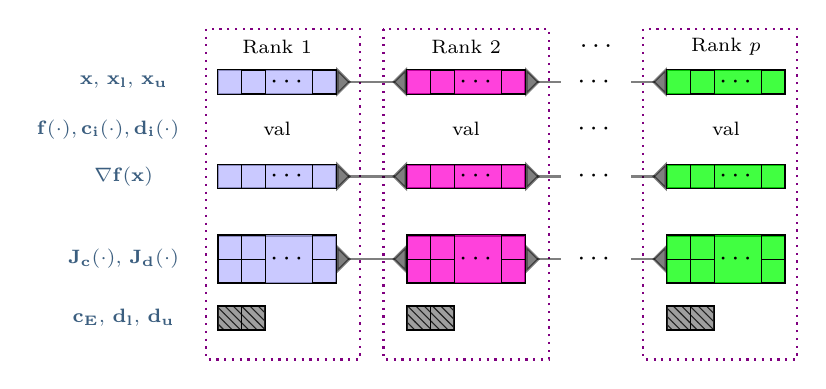
\begin{tikzpicture}[scale=.6]

%\node[inner sep=0pt] (cube) at (-7.5,-4)  {\includegraphics[width=.3\textwidth]{images/partition-2048-a}};

%\begin{scope}[every node/.append style={xslant=0.017,yslant=-0.04},xslant=0.017,yslant=-0.04]
%  %\shade[right color=gray!10, left color=black!50, semitransparent] (-10.5,-2.5) rectangle +(4,1);
%  \node[anchor=center] at (-8.,-3.75) {{\color{white} \textbf{Material and \ \ \ }}};
%  \node[anchor=center] at (-8.75,-4.35) {{\color{white} \textbf{design domain}}};
%\end{scope}

%\node[anchor=center,rotate=20,opaque=0.7] at (7.5,-4.75) {\large\color{subsecblue}\textbf{Optimization computational layout}};

%the table lines
\draw[thick,dotted,violet](2.25,0.375) rectangle+(3.25,-7.);
\draw[thick,dotted,violet](6.,0.375) rectangle+(3.5,-7.);
\draw[thick,dotted,violet](11.5,0.375) rectangle+(3.25,-7.); 

% line with procs
\draw[thick](3.75,0) node(proc1)[anchor=center]{\scriptsize Rank $1$};
\draw[thick](7.75,0) node(proc2){\scriptsize Rank $2$};
\draw[thick](10.5,0) node{$\ldots$ };
\draw[thick](13.25,0) node(procp){\scriptsize Rank $p$};


%arrowsfrom 3d-domain to procs

%\node(n1) at (-10.75,-1){};
%\node(n2) at (-7.75,-1){};
%\node(n3) at (-3.95,-5.15){};
%\path[every node/.style={font=\sffamily\small},semitransparent,gray]
%    (n1) edge[bend left,dashed,->,>=triangle 60,out=20, in=155] node [right] {} (proc1)
%    (n2) edge[bend left,dashed,->,>=triangle 60,out=20, in=155] node [right] {} (proc2)
%		(n3) edge[bend left,dashed,->,>=triangle 60,out=60, in=150] (procp);


%\draw[thick](n1) -- (proc1);

%Decision variable
%!\draw(1.,-0.75) node[anchor=center]{\color{secblue}{\textbf{\scriptsize Decision $\textbf{x}$}}};
\draw(0.5,-0.75) node[anchor=center]{\color{secblue}{\scriptsize $\mathbf{x}$, $\mathbf{x_l}$, $\mathbf{x_u}$ }};
\draw[thick](2.5,-1) rectangle+(2.5,0.5); \fill[mycolor1,fill opacity=0.75](2.5,-1) rectangle+(2.5,0.5); 
\draw(3.0,-1) rectangle +(.5,0.5);
\draw[thick](4.0,-0.75) node[anchor=center]{$\cdots$}; 
\draw(4.5,-1) rectangle+(.5,0.5);
\draw [<->, >=triangle 90 reversed, line width=0.2ex,semitransparent](5.,-.75) -- ++(1.5,0);

\draw[thick](6.5,-1) rectangle+(2.5,0.5); \fill[mycolor2,fill opacity=0.75](6.5,-1) rectangle+(2.5,0.5); 
\draw(7.0,-1) rectangle +(.5,0.5);
\draw[thick](8.0,-0.75) node[anchor=center]{$\cdots$}; 
\draw(8.5,-1) rectangle+(.5,0.5);
\draw [<-, >=triangle 90 reversed, line width=0.2ex,semitransparent](9,-0.75) -- ++(0.75,0);

\draw[thick](10.5,-0.75) node[anchor=center]{$\cdots$};
\draw [->, >=triangle 90 reversed, line width=0.2ex,semitransparent](11.25,-0.75) -- ++(0.75,0);


\draw[thick](12,-1) rectangle+(2.5,0.5); \fill[mycolor3,fill opacity=0.75](12,-1) rectangle+(2.5,0.5); 
\draw(12.5,-1) rectangle +(.5,0.5);
\draw[thick](13.5,-0.75) node[anchor=center]{$\cdots$}; 
\draw(14,-1) rectangle+(.5,0.5);

%f(x)
%\draw(0.75,-1.65) node[anchor=center]{{\footnotesize Objective \&} };
%\draw(0.75,-1.85) node[anchor=center]{{\footnotesize constraints} };
%!\draw(0.95,-1.75) node[anchor=center]{\color{secblue}{\scriptsize $\mathbf{f(x), g_i(x)}$ } };
\draw(0.25,-1.75) node[anchor=center]{\color{secblue}{\scriptsize $\mathbf{f(\cdot), c_i(\cdot), d_i(\cdot)}$ } };


%\draw[decorate,decoration={brace,mirror, amplitude=7pt},xshift=0pt,yshift=0pt]
%(2.5,-1.125) -- (5.0,-1.125) node [black,midway,yshift=-12.5pt] 
%{\scriptsize $f(x)$};
\draw(3.75,-1.75) node[anchor=center] {\scriptsize val};
\draw(7.75,-1.75) node[anchor=center] {\scriptsize val};
\draw[thick](10.5,-1.75) node[anchor=center]{$\cdots$};
\draw(13.25,-1.75) node[anchor=center] {\scriptsize val};

%\draw[decorate,decoration={brace,mirror, amplitude=7pt},xshift=0pt,yshift=0pt]
%(6.5,-1.75) -- (9.0,-1.125) node [black,midway,yshift=-12.5pt] 
%%!{\scriptsize $f_2(x_2)$};
%{\scriptsize $f(x)$};
%
%\draw[thick](10.5,-1.75) node[anchor=center]{$\cdots$};%
%
%\draw[decorate,decoration={brace,mirror, amplitude=7pt},xshift=0pt,yshift=0pt]
%(12.00,-1.125) -- (14.5,-1.125) node [black,midway,yshift=-12.5pt] 
%%!{ \scriptsize $f_p(x_p)$};
%{ \scriptsize $f_p(z_p)$};





%gradients
%\draw(0.75,-2.63) node[anchor=center]{{\footnotesize Gradients}};
%\draw(0.75,-3.02) node[anchor=center]{{\footnotesize $\nabla f(x)$, $\nabla g_i(x)$}};
%!\draw(0.7,-2.75) node[anchor=center]{\color{secblue}{\scriptsize $\mathbf{\nabla f(x), \nabla g_i(x)}$}};
\draw(0.5,-2.75) node[anchor=center]{\color{secblue}{\scriptsize $\mathbf{\nabla f(x)}$}};

\draw[thick](2.5,-3.0) rectangle+(2.5,0.5); \fill[mycolor1,fill opacity=0.75](2.5,-3.0) rectangle+(2.5,0.5); 
\draw(3.0,-3) rectangle +(.5,0.5);
\draw[thick](4.0,-2.75) node[anchor=center]{$\cdots$}; 
\draw(4.5,-3) rectangle+(.5,0.5);
\draw [<->, >=triangle 90 reversed, line width=0.2ex,semitransparent](5.,-2.75) -- ++(1.5,0);

\draw[thick](6.5,-3) rectangle+(2.5,0.5);\fill[mycolor2,fill opacity=0.75](6.5,-3) rectangle+(2.5,0.5);
\draw(7.0,-3) rectangle +(.5,0.5);
\draw[thick](8.0,-2.75) node[anchor=center]{$\cdots$}; 
\draw(8.5,-3) rectangle+(.5,0.5);
\draw [<-, >=triangle 90 reversed, line width=0.2ex,semitransparent](9,-2.75) -- ++(0.75,0);

\draw[thick](10.5,-2.75) node[anchor=center]{$\cdots$};
\draw [->, >=triangle 90 reversed, line width=0.2ex,semitransparent](11.25,-2.75) -- ++(0.75,0);

\draw[thick](12,-3) rectangle+(2.5,0.5); \fill[mycolor3,fill opacity=0.75](12,-3) rectangle+(2.5,0.5); 
\draw(12.5,-3) rectangle +(.5,0.5);
\draw[thick](13.5,-2.75) node[anchor=center]{$\cdots$}; 
\draw(14,-3) rectangle+(.5,0.5);

%Jacobians
\draw(0.5,-4.5) node[anchor=center]{\color{secblue}{\scriptsize $\mathbf{J_c(\cdot)}$, $\mathbf{J_d(\cdot)}$}};

%U
\draw[thick](2.5,-4) rectangle+(2.5,-1); \fill[mycolor1,fill opacity=0.75](2.5,-4) rectangle+(2.5,-1); 
\draw(3.0,-4) rectangle+(0.5,-0.5); \draw(3.0,-4.5)rectangle+(0.5,-0.5);
\draw(2.5,-4) rectangle+(0.5,-0.5); \draw(2.5,-4.5)rectangle+(0.5,-0.5);
%\draw(2.5,-4) grid[step=0.5]+(1,-1);
\draw[thick](4.0,-4.5) node[anchor=center]{$\cdots$}; 
\draw(4.5,-4) rectangle+(0.5,-0.5);
\draw(4.5,-4.5)rectangle+(0.5,-0.5);
%\node at(1.4,-4.5) [right,fill=green,opacity=.0,text opacity=1] {\color{secblue}{\scriptsize $\mathbf{U}$}};
\draw [<->, >=triangle 90 reversed, line width=0.2ex,semitransparent](5.,-4.5) -- ++(1.5,0);

\draw[thick](6.5,-4) rectangle+(2.5,-1); \fill[mycolor2,fill opacity=0.75](6.5,-4) rectangle+(2.5,-1);
\draw(7.0,-4) rectangle+(0.5,-0.5); \draw(7.0,-4.5)rectangle+(0.5,-0.5);
\draw(6.5,-4) rectangle+(0.5,-0.5); \draw(6.5,-4.5)rectangle+(0.5,-0.5);
%\draw(6.5,-4) grid[step=0.5]+(1,-1);
\draw[thick](8.0,-4.5) node[anchor=center]{$\cdots$}; 
\draw(8.5,-4) rectangle+(0.5,-0.5);
\draw(8.5,-4.5)rectangle+(0.5,-0.5);
\draw [<-, >=triangle 90 reversed, line width=0.2ex,semitransparent](9,-4.5) -- ++(0.75,0);

\draw[thick](10.5,-4.5) node[anchor=center]{$\cdots$};
\draw [->, >=triangle 90 reversed, line width=0.2ex,semitransparent](11.25,-4.5) -- ++(0.75,0);

\draw[thick](12,-4) rectangle+(2.5,-1);  \fill[mycolor3,fill opacity=0.75](12,-4) rectangle+(2.5,-1); 
\draw(12.0,-4) rectangle+(0.5,-0.5); \draw(12.0,-4.5)rectangle+(0.5,-0.5);
\draw(12.5,-4) rectangle+(0.5,-0.5); \draw(12.5,-4.5)rectangle+(0.5,-0.5);
%\draw(12,-4) grid[step=0.5]+(1,-1);
\draw[thick](13.5,-4.5) node[anchor=center]{$\cdots$}; 
\draw(14,-4) rectangle+(0.5,-0.5);
\draw(14,-4.5)rectangle+(0.5,-0.5);

%V
\draw(0.5,-5.75) node[anchor=center] {\color{secblue}{\scriptsize $\mathbf{c_E}$, $\mathbf{d_l}$, $\mathbf{d_u}$ }};
\draw[thick,pattern=north west lines] (2.5,-5.5) rectangle++(1,-0.5); \fill[semitransparent,darkgray] (2.5,-5.5) rectangle++(1,-0.5);\draw (2.5,-5.5) grid[step=0.5]+(1,-.5);
\draw[thick,pattern=north west lines] (6.5,-5.5) rectangle++(1,-0.5); \fill[semitransparent,darkgray] (6.5,-5.5) rectangle++(1,-0.5);\draw (6.5,-5.5) grid[step=0.5]+(1,-0.5); 
\draw[thick,pattern=north west lines] (12,-5.5) rectangle++(1,-0.5); \fill[semitransparent,darkgray] (12,-5.5) rectangle++(1,-0.5);\draw (12,-5.5) grid[step=0.5]+(1,-0.5);

%B0
%\node at(1.0,-7.25) [right,fill=green,opacity=.0,text opacity=1] {\color{secblue}{ \scriptsize $\mathbf{B_0}$} };
%\draw[thick](2.5,-7.5) rectangle+(2.5,0.5); \fill[mycolor1,fill opacity=0.75](2.5,-7.5) rectangle+(2.5,0.5); 
%\draw(3.0,-7.5) rectangle +(.5,0.5);
%\draw[thick](4.0,-7.25) node[anchor=center]{$\cdots$}; 
%\draw(4.5,-7.5) rectangle+(.5,0.5);
%\draw [<->, >=triangle 90 reversed, line width=0.2ex,semitransparent](5.,-7.25) -- ++(1.5,0);

%\draw[thick](6.5,-7.5) rectangle+(2.5,0.5); \fill[mycolor2,fill opacity=0.75](6.5,-7.5) rectangle+(2.5,0.5);
%\draw(7.0,-7.5) rectangle +(.5,0.5);
%\draw[thick](8.0,-7.25) node[anchor=center]{$\cdots$}; 
%\draw(8.5,-7.5) rectangle+(.5,0.5);
%\draw [<-, >=triangle 90 reversed, line width=0.2ex,semitransparent](9,-7.25) -- ++(0.75,0);

%\draw[thick](10.5,-7.25) node[anchor=center]{$\cdots$};
%\draw [->, >=triangle 90 reversed, line width=0.2ex,semitransparent](11.25,-7.25) -- ++(0.75,0);

%\draw[thick](12,-7.5) rectangle+(2.5,0.5); \fill[mycolor3,fill opacity=0.75](12,-7.5) rectangle+(2.5,0.5); 
%\draw(12.5,-7.5) rectangle +(.5,0.5);
%\draw[thick](13.5,-7.25) node[anchor=center]{$\cdots$}; 
%\draw(14,-7.5) rectangle+(.5,0.5);

\end{tikzpicture}
}



%\end{document}


\warningcp{Note:} All the \texttt{eval\_} functions of the C++ interface provides local array slices of the above mentioned distributed data to the application code that implements \Hi's C++ interface. The size of these local slices is the ``local size'' (specified by the application code through the \texttt{get\_vecdistrib\_info} method explained below) and is different from the ``global size'' $n$ and parameter \texttt{n} of methods. 

\warningcp{Note:} Since the Jacobians are distributed column-wise, the implementer should populate the \texttt{Jac} argument of \texttt{eval\_Jac\_cons} with the ``local'' columns.

On the other hand, the problem's data that does not have storage depending on $n$, is not distributed; instead, it is replicated on all ranks. Such data consist of $c_E$, $d_l$, $d_u$ and the evaluations of $c(x)$ and $d(x)$.
 
\begin{lstlisting} 
bool get_MPI_comm(MPI_Comm& comm_out) ;
\end{lstlisting}

\noindent Use this method to specify the MPI communicator to be used by \Hi. It has a default implementation that will provide \texttt{MPI\_COMM\_WORLD}.


%\noindent  \begin{verbatim}bool get_vecdistrib_info(size_type global_n, size_type* cols) \end{verbatim}
\begin{lstlisting}
bool get_vecdistrib_info(size_type global_n, size_type* cols);
\end{lstlisting}

\noindent Use this method to specify the data distribution of the data of the problem that has storage depending on $n$. \Hi will call the implementation of this method to obtain the partitioning/distribution of an hypothetical vector of size \texttt{global\_n} across the MPI ranks. The array \texttt{cols} is of dimension number of ranks plus one and should be populated such that \texttt{cols[r]} and \texttt{cols[r+1]-1} specify the start and end indexes of the slice stored on rank $r$ in the hypothetical vector.  It has a default implementation that will returns \texttt{false}, indicating that \Hi should run in serial.


\warningcp{Note:}  \Hi also uses \texttt{get\_vecdistrib\_info} to obtain the information about the Jacobians' distribution across MPI ranks (this is possible since they are  column-wise distributed).

Examples of how to use these functions can be found in the standalone drivers in \texttt{src/Drivers/} under the \Hi's root directory.

%\subsubsection{Additional interface methods}
%\Hi's C++ interface provides methods to retrieve the optimal solution and the intermediate iterates.

\subsubsection{Calling \Hi for a \texttt{hiopInterfaceDenseConstraints} formulation}
Once an implementation of the \texttt{hiop::hiopInterfaceDenseConstraints} abstract interface class containing the user's NLP representation is available, the  user code needs to create a \Hi problem formulation that encapsulate the NLP representation, instantiate an optimization algorithm class, and start the numerical optimization process. Assuming that the NLP representation is implemented in a class named \texttt{NlpEx1} (deriving \texttt{hiop::hiopInterfaceDenseConstraints}), the aforementioned sequence of steps can be performed by:
\begin{lstlisting}
#include "NlpEx1.hpp"               //the NLP representation class
#include "hiopInterface.hpp"   //HiOP encapsulation of the NLP
#include "hiopAlgFilterIPM.hpp"     //solver class
using namespace hiop;
...
NlpEx1 nlp_interface();                     //instantiate your NLP representation class
hiopNlpDenseConstraints nlp(nlp_interface); //create HiOP encapsulation
nlp.options.SetNumericValue("mu0", 0.01);  //set initial value for  barrier parameter
hiopAlgFilterIPM solver(&nlp);             //create a solver object
hiopSolveStatus status = solver.run();     //numerical optimization
double obj_value = solver.getObjective();  //get objective
...
\end{lstlisting}
Various output quantities of the numerical optimization phase (\textit{e.g.}, the optimal objective value and (primal) solution, status of the numerical optimization process, and solve statistics) can be retrieved from \Hi's \texttt{hiopAlgFilterIPM} solver object. Most commonly used such methods are: 
\begin{lstlisting}
double getObjective() const;
void getSolution(double* x) const;
hiopSolveStatus getSolveStatus() const;
int getNumIterations() const;
\end{lstlisting} 
The standalone drivers \texttt{nlpDenseCons\_ex1}, \texttt{nlpDenseCons\_ex2}, and \texttt{nlpDenseCons\_ex3} inside directory \texttt{src/Drivers/} under the \Hi's root directory contain more detailed examples of the use of \Hi.

%%%%%%%%%%%%%%%%%%%%%%%%%%%%%%%%%%%%%%%%%%%%%%%%%%%%%%%%%%%%%%%%%%
%%%%%%%%%%%%%%%%%%%%%%%%%%%%%%%%%%%%%%%%%%%%%%%%%%%%%%%%%%%%%%%%%%
%% NLP Sparse
%%%%%%%%%%%%%%%%%%%%%%%%%%%%%%%%%%%%%%%%%%%%%%%%%%%%%%%%%%%%%%%%%%
%%%%%%%%%%%%%%%%%%%%%%%%%%%%%%%%%%%%%%%%%%%%%%%%%%%%%%%%%%%%%%%%%%
\subsection{General sparse NLPs requiring \textit{up to second-order} derivative information}
The sparse NLP formulation supports sparse optimization problems and requires Hessians of the objective and constraints in addition to gradients/Jacobian of the objective/constraints.
\begin{align}
&&&&\min_{x\in\mathbb{R}^n} & \hspace{0.5cm} f(x) &&&& \label{spobj}\\
&&&&\textnormal{s.t.} &\hspace{0.5cm}  c(x)=c_E &[y_c]&&&\\
&&[v_l]&&& \hspace{0.5cm} d_l \leq d(x) \leq d_u  &[v_u]&&&\label{spineq} \\
&&[z_u]&&& \hspace{0.5cm} x_l \leq x \leq x_u & [z_u] &&&\label{spbounds}
\end{align}
Here $f:\mathbb{R}^n\rightarrow\mathbb{R}$, $c:\mathbb{R}^n\rightarrow\mathbb{R}^{m_E}$, $d:\mathbb{R}^n\rightarrow\mathbb{R}^{m_I}$. The bounds appearing in the inequality constraints~\eqref{ineq} are assumed to be $d^l\in\mathbb{R}^{m_I}\cup\{-\infty\}$, $d^u\in\mathbb{R}^{m_I}\cup\{+\infty\}$, $d_i^l < d_i^u$, and at least of one of $d_i^l$ and $d_i^u$ are finite for all $i\in\{1,\ldots,m_I\}$. The bounds in~\eqref{bounds} are such that $x^l\in\mathbb{R}^{n}\cup\{-\infty\}$, $x^u\in\mathbb{R}^{n}\cup\{+\infty\}$, and $x_i^l < x_i^u$, $i\in\{1,\ldots,n\}$. The quantities insides brackets are the Lagrange multipliers of the constraints. Whenever a bound is infinite, the corresponding multiplier is by convention zero.

The following quantities are required by \Hi:
\begin{itemize}
\item[D1] objective and constraint functions $f(x)$, $c(x)$, $d(x)$;
\item[D2] the first-order derivatives of the above: $\nabla f(x)$, $Jc(x)$, $Jd(x)$;
\item[D3] The Hessian of the Lagrangian
  \begin{align}
\nabla^2 L(x)& = \lambda_0 \nabla^2 f(x) + \sum_{i=1}^{m_E} \lambda_i^E \nabla^2 c_i(x) + \sum_{i=1}^{m_I} \lambda_i^I \nabla^2 d_i(x).\label{spHess}
\end{align}
\item[D4] the simple bounds $x_l$ and $x_u$, the inequalities bounds: $d_l$ and $d_u$, and the right-hand size of the equality constraints $c_E$.
\end{itemize}

\subsubsection{C++ interface to solve sparse NLPs}
The above optimization problem~\eqref{spobj}-\eqref{spbounds} can be specified by using the C++ interface, namely by deriving and providing an implementation for the \texttt{hiop::hiopInterfaceSparse} abstract class.

 We present next the methods of this abstract class that needs to be implemented in order to specify the parts D1-D4 required to solve a sparse NLP  problem. 

\warningcp{Note:} All the functions that have a \texttt{bool} return type should return \texttt{false} when an error occurs, otherwise should return \texttt{true}.

\warningcp{Note:} \texttt{hiop::hiopInterfaceSparse} runs only in non-distributed/non-MPI mode. Intraprocess acceleration can be obtained using OpenMP or CUDA.

\subsubsection{Specifying the optimization problem}

All the methods of this section are ``pure'' virtual in \texttt{hiop::hiopInterfaceSparse} abstract class  and need to be provided by the user implementation.

\begin{lstlisting} 
bool get_prob_sizes(long long& n, long long& m);
\end{lstlisting} 
\noindent Provides the number of decision variables and the number of constraints ($m=m_E+m_I$).


\begin{lstlisting} 
bool get_vars_info(const long long& n, double *xlow, double* xupp, 
                   NonlinearityType* type);
\end{lstlisting} 

\noindent Provides the lower and upper bounds $x_l$ and $x_u$ on the decision variables. When a variable (let us say the $i^{th}$) has no lower or/and upper bounds, the  $i^{th}$ entry of xlow and/or xupp should be less than $-1e20$ or/and larger than $1e20$, respectively. The last argument is not used and can set to any value of the enum \texttt{hiop::hiopInterface::NonlinearityType}.

\begin{lstlisting} 
bool get_cons_info(const long long& m, double* clow, double* cupp, 
                   NonlinearityType* type);
\end{lstlisting}
\noindent Similar to the above, but for the inequality bounds $d_l$ and $d_u$. For equalities, set the corresponding entries in clow and cupp equal to the desired value (from $c_E$).


\begin{lstlisting} 
bool eval_f(const long long& n, 
            const double* x, bool new_x, 
            double& obj_value);
\end{lstlisting} 

\noindent Implement this method to compute the function value $f(x)$ in \texttt{obj\_value} for the provided decision variables $x$. The input argument \texttt{new\_x} specifies whether the variables $x$ have been changed since the previous call of one of the \texttt{eval\_} methods. Use this argument to ``buffer'' the objective and gradients function and derivative evaluations when this is possible.

\begin{lstlisting} 
bool eval_grad_f(const long long& n, 
                 const double* x, bool new_x, 
                 double* gradf);
\end{lstlisting} 

\noindent Same as above but for $\nabla f(x)$.

%%%%%%%%%%%%%%%%%%%%%%%%%%%%%%%%%%%%%%%%%%%%%%
\begin{lstlisting} 
 bool eval_cons(const long long& n, const long long& m, 
                const long long& num_cons,
				    const long long* idx_cons, const double* x, 
			       bool new_x, double* cons);
\end{lstlisting} 

\noindent Implement this method to provide the value of the constraints $c(x)$ and/or $d(x)$. The input parameter \texttt{num\_cons} specifies how many constraints (out of \texttt{m}) needs to evaluated; \texttt{idx\_cons} array specifies the indexes, which are zero-based, of the constraints  and is of size \texttt{num\_cons}. These values should be provided in \texttt{cons}, which is also an array of size \texttt{num\_cons}.
%%%%%%%%%%%%%%%%%%%%%%%%%%%%%%%%%%%%%%%%%%%%%%



\begin{lstlisting} 
bool 
eval_Jac_cons(const long long& n, const long long& m, 
			     const long long& num_cons, const long long* idx_cons,  
			     const double* x, bool new_x,
			     const int& nnzJacS, int* iJacS, int* jJacS, double* MJacS);
\end{lstlisting} 

\noindent Implement this method to provide the Jacobian of a subset of the  constraints $c(x)$ and/or $d(x)$ in \texttt{Jac}; this subset is specified by the array \texttt{idx\_cons}. The last three arguments should be used to specify the Jacobian information in sparse triplet format.  \texttt{iJacS} and \texttt{jJacS} needs to be jointly sorted: by indexes in \texttt{iJacS} and, for equal (row) indexes in \texttt{iJacS}, by indexes in \texttt{jJacS}.

Notes for implementer of this method: 
\begin{itemize}
\item[2.] When \texttt{iJacS} and \texttt{jJacS} are non-null, the implementer should provide the $(i,j)$   indexes in these arrays. 
\item[3.] When \texttt{MJacS} is non-null, the implementer should provide the values corresponding to    entries specified by \texttt{iJacS} and \texttt{jJacS}.
\item[4.] \texttt{iJacS} and \texttt{jJacS} are both either non-null or null during the same call.
\item[5.] The pair (\texttt{iJacS}, \texttt{jJacS}) and \texttt{MJacS} can be both non-null during the same call or only one of them  non-null; but they will not be both null.
\end{itemize}
%%%%%%%%%%%%%%%%%%%%%%%%%%%%%%%%%%%%%%%%%%%%%%

%%%%%%%%%%%%%%%%%%%%%%%%%%%%%%%%%%%%%%%%%%%%%%
\begin{lstlisting}
bool eval_Jac_cons(const long long& n, const long long& m, 
			          const double* x, bool new_x,
			          const int& nnzJacS, int* iJacS, int* jJacS, double* MJacS);
\end{lstlisting} 

\noindent Evaluates the Jacobian of equality and inequality constraints \textit{in one call}. 
   
\warningcp{Note:}   HiOp will call this method whenever the implementer/user returns \texttt{false} from the previous, ``two-calls'' \texttt{eval\_Jac\_cons}. We remark that the two-calls method should return  \texttt{false} during both calls (for equalities and inequalities) made to it by \Hi in order to let \Hi know that the Jacobian should be evaluated using the one-call callback listed above.
   
   
   
The main difference from the above \texttt{eval\_Jac\_cons} is that the implementer/user of this 
    method does not have to split the constraints into equalities and inequalities; instead,
    HiOp does this internally.
   
 
   Parameters:
    \begin{itemize}
    \item  first four: number of variables, number of constraints, (primal) variables at which the
    Jacobian should be evaluated, and boolean flag indicating whether the variables \texttt{x} have
    changed since a previous call to any of the function and derivative evaluations.
     \item   \texttt{nnzJacS}, \texttt{iJacS}, \texttt{jJacS}, \texttt{MJacS}: number of nonzeros, $(i,j)$ indexes, and nonzero values of 
   the sparse Jacobian matrix.  \texttt{iJacS} and \texttt{jJacS} needs to be jointly sorted: by indexes in \texttt{iJacS} and, for equal (row) indexes in \texttt{iJacS}, by indexes in \texttt{jJacS}.
    \end{itemize}
   
\warningcp{Note:} Notes 1-5 from the previous, two-call \texttt{eval\_Jac\_cons} applies here as well.

%%%%%%%%%%%%%%%%%%%%%%%%%%%%%%%%%%%%%%%%%%%%%%


%%%%%%%%%%%%%%%%%%%%%%%%%%%%%%%%%%%%%%%%%%%%%%
\begin{lstlisting} 
bool eval_Hess_Lagr(const long long& n, const long long& m, 
			      const double* x, bool new_x, const double& obj_factor,
			      const double* lambda, bool new_lambda,
			      const long long& nsparse, const long long& ndense, 
			      const int& nnzHSS, int* iHSS, int* jHSS, double* MHSS)
\end{lstlisting} 

\noindent Evaluates the Hessian of the Lagrangian function as a sparse matrix in triplet format. 

 
 
\warningcp{Note:} Notes 1-5 from \texttt{eval\_Jac\_cons} apply to arrays \texttt{iHSS}, \texttt{jHSS}, and \texttt{MHSS} that stores the sparse part of the Hessian.

\warningcp{Note:} The array \texttt{lambda} contains first the multipliers of the equality constraints followed by the multipliers of the inequalities.

%%%%%%%%%%%%%%%%%%%%%%%%%%%%%%%%%%%%%%%%%%%%%%

\subsubsection{Calling \Hi for a \texttt{hiopInterfaceSparse} formulation}
Once the sparse NLP is coded,  the  user code needs to create a \Hi problem formulation that encapsulate the NLP representation, instantiate an optimization algorithm class, and start the numerical optimization process. Assuming that the NLP representation is implemented in a class named \texttt{NlpEx6} (that derives from \texttt{hiop::hiopInterfaceSparse}), the aforementioned sequence of steps can be performed by:
\begin{lstlisting}
#include "NlpEx6.hpp"               //the NLP representation class
#include "hiopInterface.hpp"   //HiOP encapsulation of the NLP
#include "hiopAlgFilterIPM.hpp"     //solver class
using namespace hiop;
...
NlpEx6 nlp_interface();                     //instantiate your NLP representation class
hiopNlpDenseConstraints nlp(nlp_interface); //create HiOP encapsulation
nlp.options.SetNumericValue("mu0", 0.01);  //set a non-default initial value for  barrier parameter
hiopAlgFilterIPM solver(&nlp);             //create a solver object
hiopSolveStatus status = solver.run();     //numerical optimization
double obj_value = solver.getObjective();  //get objective
...
\end{lstlisting}
Various output quantities of the numerical optimization phase (\textit{e.g.}, the optimal objective value and (primal) solution, status of the numerical optimization process, and solve statistics) can be retrieved from \Hi's \texttt{hiopAlgFilterIPM} solver object. Most commonly used such methods are: 
\begin{lstlisting}
double getObjective() const;
void getSolution(double* x) const;
hiopSolveStatus getSolveStatus() const;
int getNumIterations() const;
\end{lstlisting} 
The standalone drivers \texttt{nlpSparse\_ex6} and \texttt{nlpSparse\_ex7} inside directory \texttt{src/Drivers/} under the \Hi's root directory contain more detailed examples of the use of the sparse NLP interface of \Hi.


%%%%%%%%%%%%%%%%%%%%%%%%%%%%%%%%%%%%%%%%%%%%%%%%%%%%%%%%%%%%%%%%%%
%%%%%%%%%%%%%%%%%%%%%%%%%%%%%%%%%%%%%%%%%%%%%%%%%%%%%%%%%%%%%%%%%%
%% NLP MDS
%%%%%%%%%%%%%%%%%%%%%%%%%%%%%%%%%%%%%%%%%%%%%%%%%%%%%%%%%%%%%%%%%%
%%%%%%%%%%%%%%%%%%%%%%%%%%%%%%%%%%%%%%%%%%%%%%%%%%%%%%%%%%%%%%%%%%
\subsection{NLPs in the mixed dense-sparse (MDS) form}\label{sec:mds}
A second class of optimization problems supported by \Hi consists of nonlinear, possibly nonconvex optimization problems that explicitly partition the optimization variables into so-called ``dense'' and ``sparse'' variables, $x_d$ and $x_s$, respectively; this problem can be  expressed compactly as
\begin{align}
\min_{x_d\in\mathbb{R}^{n_d}, x_s\in\mathbb{R}^{n_s}} & \hspace{0.3cm} f(x_d, x_s) && \label{mdsobj}\\
\textnormal{s.t.} &\hspace{0.3cm}  c(x_d, x_s)=c_E, &&\\
 &\hspace{0.3cm} d^l \leq d(x_d, x_s) \leq d^u,  &&\label{mdsineq} \\
 &\hspace{0.3cm} x^{l}_{d} \leq x_d \leq x^{u}_{d}, \ x^{l}_{s} \leq x_s \leq x^{u}_{s}. &&\label{mdsbounds}
\end{align}
Here $f:\mathbb{R}^n\rightarrow\mathbb{R}$, $c:\mathbb{R}^n\rightarrow\mathbb{R}^{m_E}$, and $d:\mathbb{R}^n\rightarrow\mathbb{R}^{m_I}$, where $n$ denotes the total number of variables, $n=n_d + n_s$. The bounds appearing in the inequality constraints~\eqref{mdsineq} are assumed to be $d^l\in\mathbb{R}^{m_I}\cup\{-\infty\}$, $d^u\in\mathbb{R}^{m_I}\cup\{+\infty\}$, $d_i^l < d_i^u$, and at least of one of $d_i^l$ and $d_i^u$ are finite for each $i\in\{1,\ldots,m_I\}$. The vector bounds $x^{l}_{d}$, $x^{u}_{d}$, $x^{l}_{s}$, and $x^{u}_{s}$ in~\eqref{mdsbounds} need to satisfy identical requirements.  
For the rest of the paper $m$ will denote $m_E+m_I$, \textit{i.e.}, the total number of constraints excepting the simple bounds constraints~\eqref{mdsbounds}.

The salient idea behind mixed dense-sparse problems of the form~\eqref{mdsobj}-\eqref{mdsbounds} is that the explicit partitioning of the optimization variables and a couple of (block) structural properties of the functions $f(\cdot)$, $c(\cdot)$, and $d(\cdot)$, which are elaborated below, allow orchestrating the computations of the optimization algorithm to heavily rely on matrix and vector \textit{dense} kernels and to reduce the reliance on sparse linear algebra kernels.

As mentioned above we make a couple of assumptions on the block structure of the derivatives:
\begin{itemize}
    \item[A1.] The ``cross-term'' Hessian matrices $\nabla^2_{x_d x_s} f$, $\nabla^2_{x_s x_d} f$, $\nabla^2_{x_d x_s} c$, $\nabla^2_{x_s x_d} c$, $\nabla^2_{x_d x_s} d$, and $\nabla^2_{x_s x_d} d$ are zero;
    \item[A2.] The Hessian matrix $\nabla^2_{x_s x_s} L$ has a sparsity pattern that allows \textit{computationally efficient} inversion of (or solving with) the matrix $\nabla^2_{x_s x_s} L + D_{x_s}$ where $D_{x_s}$ is a diagonal matrix with positive diagonal entries; in our target applications, namely, optimal power flow problems, $\nabla^2_{x_s x_s} L$ is a diagonal matrix with nonnegative entries.
\end{itemize}

The optimization problem~\eqref{mdsobj}--\eqref{mdsbounds} is transformed internally by \Hi to an equivalent form that is more amenable to the use of interior-point methods as described on~\cite[Section~3]{petra2019memory}. Furthermore, HiOp implements the filter line-search interior-point algorithm of W{\"a}chter and Biegler~\cite{waecther_05_ipopt,waecther_05_ipopt2} (also implemented by IPOPT~\cite{waecther_05_ipopt0}) and makes explicit use of second-order derivatives/Hessians.

\Hi offers support for NVIDIA GPU acceleration. This feature is available only when solving NLPs in the mixed dense-sparse (MDS) form and should be enabled during the build by using \texttt{-DHIOP\_USE\_GPU} option with \texttt{cmake}. \Hi's \texttt{cmake} build system is quite versatile to find the dependencies required to offload computations to the device GPUs since was developed and tested on a few GPU-enabled HPC platforms at Oak Ridge, Lawrence Livermore, and Pacific Northwestern National Laboratories. These dependencies consist of CUDA library and Magma linear solver library.
%If offloading computations to the device is not desired, the user can switch it off and perform only CPU (host) computations by setting \Hi's option \texttt{compute\_mode} to \texttt{cpu}.
The Newton interior-point solver for MDS problems offers the possibility to perform the linear algebra and the great majority of the optimization computations on the device; this can be achieved by setting option \texttt{compute\_mode} to \texttt{gpu} and the option \texttt{mem\_space} to \texttt{device}. This combination of the two options will require the problem evaluation functions implemented by the user (see Section~\ref{sec:mds:cpp} below) to run on the device. If the user code does not support this, then \Hi should be used with \texttt{compute\_mode} set to \texttt{hybrid} and the option \texttt{mem\_space} set to \texttt{default}; this combination will offload the majority of linear algebra and optimization computations to the device. The \Hi's RAJA version of Example 4 (see \texttt{src/Drivers/nlpMDS\_ex4\_raja\_driver.cpp}) provides an example of implementing a MDS NLP so that it that can be solved by running \Hi's Newton solver on the device (\textit{i.e.}, \texttt{compute\_mode} set to \texttt{gpu} and with \texttt{mem\_space} set to \texttt{device}).

We note that MDS NLPs have no support for coarse grain (interprocess/internode) parallelism.

%After a careful manipulation of the equations, which is described in detail in~\cite{petra2019memory}, also see~\cite{wachter2006implementation}, the interior-point solver needs to perform computations that can roughly categorized as 
%\begin{itemize}
%\item vector-vector operations involving only dense vectors, for example, in updating the optimization variables along the search direction (``axpy''), computing residual norms, searching for min/max elements, etc.;
%\item matrix-vector operations involving both sparse and dense matrices and dense vectors, for example in residual computation;
%\item solving augmented MDS linear systems of the form
%\begin{align}
%    \left[\begin{array}{cccc}
%        \nabla^2_{x_s x_s} L + D_{x_s} & 0 & J_{x_s}^T c & J_{x_s}^T d  \\
%         0 & \nabla^2_{x_d x_d} L + D_{x_d} & J_{x_d}^T &  J_{x_d}^T d\\
%         J_{x_s} c & J_{x_d} c & 0 & 0 \\
%         J_{x_s} d & J_{x_d} d & 0 & D_d^{-1} \\
%    \end{array}\right]
%    \left[\begin{array}{c} \Delta x_s \\ \Delta x_d \\ \Delta y_c \\ \Delta y_d\end{array}\right] = 
%    \left[\begin{array}{c}  r_{x_s} \\ r_{x_d} \\ r_{y_c} \\  r_{y_d}\end{array}\right]
%\end{align}
%\end{itemize}

\medskip

The following quantities are required by \Hi:
\begin{itemize}
\item[D1] objective and constraint functions $f(x_d,x_s)$, $c(x_d,x_s)$, $d(x_d,x_s)$;
\item[D2] the first-order derivatives: $\nabla f(x_d,x_s)$, $Jc(x_d,x_s)$, $Jd(x_d,x_s)$; the two Jacobians will have a MDS structure in the sense that the left blocks will be dense while the right blocks will be sparse in their expressions
\begin{align}
Jc(x_d,x_s) &= \left[\begin{array}{cc} J_{x_d} c(x_d,x_s) &  J_{x_s} c(x_d,x_s)\end{array}\right] 
\end{align}
and
\begin{align}
Jd(x_d,x_s) &= \left[\begin{array}{cc} J_{x_d} d(x_d,x_s) &  J_{x_s} d(x_d,x_s)\end{array}\right]. \label{mdsJac}
\end{align}
\Hi does not track MDS structure within the gradient $\nabla f(x_d,x_s)$ and treats it as an unstructured vector.
\item[D3] the second-order derivatives in the form of the Hessian of the Lagrangian
\begin{align}
\nabla^2 L(x_d,x_s)& = \lambda_0 \nabla^2 f(x_d,x_s) + \sum_{i=1}^{m_E} \lambda_i^E \nabla^2 c_i(x_d,x_s) + \sum_{i=1}^{m_I} \lambda_i^I \nabla^2 d_i(x_d,x_s).\label{mdsHess}
\end{align}
We remark that  $\nabla^2 L(x_d,x_s)$ has a so-called MDS structure in the sense that $\nabla^2_{x_d^2} L(x_d,x_s)$ is dense, $\nabla^2_{x_s^2} L(x_d,x_s)$ is sparse, and $\nabla^2_{x_d x_s} L(x_d,x_s)$ and $\nabla^2_{x_s x_d} L(x_d,x_s)$ are zero; this is a consequence of the assumptions A1 and A2 above,

\item[D4] the simple bounds $x_l$ and $x_u$, the inequalities bounds: $d_l$ and $d_u$, and the right-hand size of the equality constraints $c_E$.
\end{itemize}

\subsubsection{The C++ interface}\label{sec:mds:cpp}
The above optimization problem~\eqref{mdsobj}--\eqref{mdsbounds} can be specified by using the C++ interface, namely by deriving and providing an implementation for the \texttt{hiop::hiopInterfaceMDS} abstract class.

 We present next the methods of this abstract class that needs to be implemented in order to specify the parts D1-D4 of the optimization problem. All the methods of this section are ``pure'' virtual in \texttt{hiop::hiopInterfaceMDS} abstract class  and need to be provided by the user implementation.
 
 

\warningcp{Note:} Unless stated otherwise, all the functions that return \texttt{bool} should return \texttt{false} when an error occurs, otherwise should return \texttt{true}.

\begin{lstlisting} 
bool get_prob_sizes(size_type& n, size_type& m);
\end{lstlisting} 
\noindent Provides the number of decision variables and the number of constraints ($m=m_E+m_I$).


\begin{lstlisting} 
bool get_vars_info(const size_type& n, double *xlow, double* xupp, 
                   NonlinearityType* type);
\end{lstlisting} 

\noindent Provides the lower and upper bounds $x_l$ and $x_u$ on the decision variables. When a variable (let us say the $i^{th}$) has no lower or/and upper bounds, the  $i^{th}$ entry of xlow and/or xupp should be less than $-1^{20}$ or/and larger than $1^{20}$, respectively. The last argument is not used and can set to any value of the enum \texttt{hiop::hiopInterfaceDenseConstraints::NonlinearityType}.


\begin{lstlisting} 
bool get_cons_info(const size_type& m, double* clow, double* cupp, 
                   NonlinearityType* type);
\end{lstlisting}
\noindent Similar to the above, but for the inequality bounds $d_l$ and $d_u$. For equalities, set the corresponding entries in clow and cupp equal to the desired value (from $c_E$).

\begin{lstlisting} 
bool get_sparse_dense_blocks_info(int& nx_sparse, int& nx_dense,
					                   int& nnz_sparse_Jaceq, 
					                   int& nnz_sparse_Jacineq,
					                   int& nnz_sparse_Hess_Lagr_SS, 
					                   int& nnz_sparse_Hess_Lagr_SD);
\end{lstlisting}
\noindent Specifies the number of nonzero elements in the  \textit{sparse blocks} of the Jacobians of the constraints and of the Hessian of the Lagrangian, see~\eqref{mdsJac} and~\eqref{mdsHess}, respectively. The last parameter \texttt{nnz\_sparse\_Hess\_Lagr\_SD} is not used momentarily and should be set to zero.

\begin{lstlisting} 
bool eval_f(const size_type& n, 
            const double* x, bool new_x, 
            double& obj_value);
\end{lstlisting} 

\noindent Implement this method to compute the function value $f(x)$ in \texttt{obj\_value} for the provided decision variables $x$. The input argument \texttt{new\_x} specifies whether the variables $x$ have been changed since the previous call of one of the \texttt{eval\_} methods. Use this argument to ``buffer'' the objective and gradients function and derivative evaluations when this is possible.

\begin{lstlisting} 
bool eval_grad_f(const size_type& n, 
                 const double* x, bool new_x, 
                 double* gradf);
\end{lstlisting} 

\noindent Same as above but for $\nabla f(x)$.

\begin{lstlisting} 
 bool eval_cons(const size_type& n, const size_type& m, 
                const size_type& num_cons,
		const index_type* idx_cons, const double* x, 
		bool new_x, double* cons);
\end{lstlisting} 

\noindent Implement this method to provide the value of the constraints $c(x)$ and/or $d(x)$. The input parameter \texttt{num\_cons} specifies how many constraints (out of \texttt{m}) needs to evaluated; \texttt{idx\_cons} array specifies the indexes, which are zero-based, of the constraints  and is of size \texttt{num\_cons}. These values should be provided in \texttt{cons}, which is also an array of size \texttt{num\_cons}.

\begin{lstlisting} 
eval_Jac_cons(const size_type& n, const size_type& m, 
              const size_type& num_cons, const index_type* idx_cons,
              const double* x, bool new_x,
              const size_type& nsparse, const size_type& ndense,
              const size_type& nnzJacS,
              index_type* iJacS, index_type* jJacS, double* MJacS, 
              double* JacD);
\end{lstlisting} 

%\noindent Implement this method to provide the Jacobian of a subset of the  constraints $c(x)$ and/or $d(x)$ in \texttt{Jac}; as above this subset is specified by the array \texttt{idx\_cons}. To set the $(i,j)$ entry of the Jacobian to $v$, one can use  \texttt{Jac[i][j]=v;}. Alternatively,  if you have a contiguous row-wise array storage of the Jacobian, simply (mem)copy it in \texttt{Jac[0]}. 

Evaluates the Jacobian of constraints split in the sparse (triplet format) and dense submatrices (row-wise contiguous memory storage). The methods is called by \Hi twice once for equalities and once for inequalities and passes during each of these calls  the \texttt{idx\_cons} array of the indexes of equalities and inequalities in the whole body of constraints.

It is advantageous to provide
this method when the underlying NLP's constraints come naturally split in equalities
and inequalities. When this is not convenient to do so, use \texttt{eval\_Jac\_cons} below.

Parameters:
\begin{itemize} 
\item first six: see \texttt{eval\_cons}.
\item \texttt{nnzJacS}, \texttt{iJacS}, \texttt{jJacS}, \texttt{MJacS} are for number of nonzeros, $(i,j)$ indexes, and nonzero values of   the sparse Jacobian.
\item \texttt{JacD} should contain the Jacobian with respect to the dense variables of the MDS problem. The array should store this Jacobian submatrix row-wise, meaning that the each row of the Jacobian is contiguous in memory and starts right after the previous row.
\end{itemize}

\warningcp{Note:} When implementing this method one should be aware that:
\begin{itemize}
\item[1.] \texttt{JacD} parameter will be always non-null
\item[2.] When \texttt{iJacS} and \texttt{jJacS} are non-null, the implementer should provide the $(i,j)$   indexes in these arrays. 
\item[3.] When \texttt{MJacS} is non-null, the implementer should provide the values corresponding to    entries specified by \texttt{iJacS} and \texttt{jJacS}.
\item[4.] \texttt{iJacS} and \texttt{jJacS} are both either non-null or null during a call.
\item[5.] The pair (\texttt{iJacS}, \texttt{jJacS}) and \texttt{MJacS} can be both non-null during the same call or only one of them  non-null; but they will not be both null.
\end{itemize}


\begin{lstlisting}
bool eval_Jac_cons(const size_type& n, const size_type& m, 
                   const double* x, bool new_x,
                   const size_type& nsparse, const size_type& ndense,
                   const size_type& nnzJacS,
                   index_type* iJacS, index_type* jJacS, double* MJacS,
                   double* JacD);
\end{lstlisting} 

\noindent Evaluates the Jacobian of equality and inequality constraints \textit{in one call}. This Jacobian is mixed dense-sparse (MDS), which means is structurally split in the sparse (triplet format) and dense matrices (contiguous rows storage)
   
\warningcp{Note:}   HiOp will call this method whenever the implementer/user returns \texttt{false} from the previous, two-calls \texttt{eval\_Jac\_cons}; we remark that this method should return  \texttt{false} during both calls (for equalities and inequalities) made to it by \Hi.
   
   
   
The main difference from the above \texttt{eval\_Jac\_cons} is that the implementer/user of this 
    method does not have to split the constraints into equalities and inequalities; instead,
    HiOp does this internally.
   
 
   Parameters:
    \begin{itemize}
    \item  first four: number of variables, number of constraints, (primal) variables at which the
    Jacobian should be evaluated, and boolean flag indicating whether the variables \texttt{x} have
    changed since a previous call to any of the function and derivative evaluations.
    \item   \texttt{nsparse} and \texttt{ndense}: number of sparse and dense variables, respectively, adding up to \texttt{n}.
     \item   \texttt{nnzJacS}, \texttt{iJacS}, \texttt{jJacS}, \texttt{MJacS}: number of nonzeros, $(i,j)$ indexes, and nonzero values of 
   the sparse Jacobian block; these indexes are within the sparse Jacobian block (not within 
    the entire Jacobian).
     \item  \texttt{JacD}: dense Jacobian block as a contiguous array storing the matrix by rows.
    \end{itemize}
   
\warningcp{Note:} Notes 1-5 from the previous, two-call \texttt{eval\_Jac\_cons} applies here as well.
    
\begin{lstlisting} 
bool eval_Hess_Lagr(const size_type& n, const size_type& m, 
                    const double* x, bool new_x, const double& obj_factor,
                    const double* lambda, bool new_lambda,
                    const size_type& nsparse, const size_type& ndense, 
                    const size_type& nnzHSS,
                    index_type* iHSS, index_type* jHSS, double* MHSS, 
                    double* HDD,
                    size_type& nnzHSD, index_type* iHSD, index_type* jHSD,
                    double* MHSD);
\end{lstlisting} 

\noindent Evaluates the Hessian of the Lagrangian function in three structural blocks given by the MDS structure of the problem. The arguments \texttt{nnzHSS}, \texttt{iHSS}, \texttt{jHSS}, and \texttt{MHSS} hold  $\nabla^2 L(x_s,x_s)$ from~\eqref{mdsHess}. The argument \texttt{HDD} stores $\nabla^2 L(x_d,x_d)$ from~\eqref{mdsHess}. 


\warningcp{Note:} The last four arguments, which are supposed to store the cross-Hessian $\nabla^2 L(x_s,x_d)$ from~\eqref{mdsHess}, are for now assumed to hold a zero matrix. The implementer should return \texttt{nnzHSD=0} during the first call to \texttt{eval\_Hess\_Lagr}. On subsequent calls, \Hi will pass the sparse triplet \texttt{HSD} arrays   set to \texttt{NULL} and the implementer (obviously) should not use them.
 
 
\warningcp{Note:} Notes 1-5 from \texttt{eval\_Jac\_cons} apply to arrays \texttt{iHSS}, \texttt{jHSS}, and \texttt{MHSS} storing the sparse part of the Hessian as well as to the \texttt{HDD} array storing the dense block of the Hessian. 

\warningcp{Note:} The rule of thumb is that when specifying \textit{symmetric} matrices to \Hi, only the \textit{upper triangle elements} should be specified by the user. The rule applies both to sparse and dense matrices. More info on \Hi's conventions on matrices storage can be found at \url{https://github.com/LLNL/hiop/tree/develop/src/LinAlg}.

%that sparse symmOnly upper triangular nonzero entries should be specified, accessed, and maintained. The Hessian and the symmetric KKT systems are implemented as symmetric matrices. Users only need to provide the upper triangle nonzero entries to Hessian. 

\warningcp{Note:} The array \texttt{lambda} contains  the multipliers of constraints. These multipliers come have the same order as the constraints in \texttt{eval\_cons} (this is a new behavior introduced in \Hi v0.4).

\warningcp{Device computations:} \Hi supports full device/GPU acceleration for MDS NLPs. To achieve this, the user can use option \texttt{compute\_mode} set to \texttt{gpu} and option \texttt{mem\_space} set to \texttt{device}. However, the user needs to be able to evaluate the model on the device. The rule of thumb is that all the \textit{pointer} arguments of the callback methods of this section will be on the device (with a few exceptions) so that the user can populate the arrays on the device. This is illustrated and discussed in detail in \texttt{src/Drivers/nlpMDS\_raja\_ex4.hpp}, which is part of the RAJA Example 4 (see \texttt{src/Drivers/nlpMDS\_ex4\_raja\_driver.cpp}) that is capable of running completely in the device memory space with minimal host-device transfer.

\subsubsection{Calling \Hi for a \texttt{hiopInterfaceMDS} formulation}
Once an implementation of the \texttt{hiop::hiopInterfaceMDS} abstract interface class containing the user's NLP representation is available, the  user code needs to create a \Hi problem formulation that encapsulate the NLP representation, instantiate an optimization algorithm class, and start the numerical optimization process. 

A detailed, self-contained example can be found in \texttt{src/Drivers/} directory in \texttt{nlpMDS\_ex4\_driver.cpp} files for an illustration of aforementioned sequence of steps. A synposis of \Hi code that solves and MDS NLP implemented presumably in a class \texttt{Ex4 } (implemented in \texttt{nlpMDSForm\_ex4.hpp}) derived from \texttt{hiop::hiopInterfaceMDS} is as follows:
\begin{lstlisting}
#include "nlpMDSForm_ex4.hpp"               //the NLP representation class
#include "hiopInterface.hpp"   //HiOP encapsulation of the NLP
#include "hiopAlgFilterIPM.hpp"     //solver class
using namespace hiop;
...
Ex4* my_nlp = new Ex4(n_sp, n_de); //instantiate your NLP representation class                    
hiopNlpMDS nlp(*my_nlp); //create HiOP encapsulation
nlp.options->SetStringValue("Hessian", "analytical_exact");
nlp.options->SetNumericValue("mu0", 0.01);  //set initial value for  barrier parameter
hiopAlgFilterIPMNewton solver(&nlp);         //create a solver object
hiopSolveStatus status = solver.run();     //numerical optimization
double obj_value = solver.getObjective();  //get objective
...
\end{lstlisting}


\subsection{Structured NLPs suitable to primal decomposition (PriDec) schemes}\label{sec:pridec}

Starting v0.5, \Hi also offers parallel computing capabilities via the PriDec solver for NLPs with separable objective terms in the form of:
\begin{align}
&&&&\min_{x\in\mathbb{R}^n} & \hspace{0.5cm} f(x) + \sum_{i=1}^K r_i(x) &&&& \label{prideobj}\\
&&&&\textnormal{s.t.} &\hspace{0.5cm}  c(x)=c_E,  &[y_c]&&&\\
&&[v_l]&&& \hspace{0.5cm} d_l \leq d(x) \leq d_u,  &[v_u]&&&\label{prideineq} \\
&&[z_u]&&& \hspace{0.5cm} x_l \leq x \leq x_u. & [z_u] &&&\label{pridebounds}
\end{align}
Mathematically, the above problem is identical (and has the same specification) to the NLP~\eqref{obj}-\eqref{bounds}, with the exception of the so-called ``recourse'' terms $r_i(x)$ appearing in the objective. Each of these functions are real-valued, $r_i:\mathbb{R}^n\rightarrow \mathbb{R}$, for all $i\in\{1,2,\ldots, K\}$, and can be of various order of differentiability. As of now, the recourse functions $r_i(x)$ need to be Lipschitz continuous and continuously differentiable.
It is also possible for $r_i(x)$ to be Lipschitz and only weakly concave (with convergence guarantees). The users are encouraged to contact \Hi developers for the latest developements in this area. A compact description of the algorithm implemented by PriDec can be found in~\cite{pridec_impl} (the technical report version is available \texttt{doc/} directory).

The input in which \Hi expects for this class of problems is a bit different than for NLPs of the form~\eqref{obj}-\eqref{bounds} and MDS NLPs introduced in the previous sections. This is mainly caused by the specifics of the primal decomposition algorithm/solver that was purposedly developed to solve~\eqref{prideobj}-\eqref{pridebounds} for large $K$ (\textit{e.g.}, $K=O(10^6)$) efficiently on a massively parallel computing platform. Nevertheless, for smaller $K$, problems of form~\eqref{prideobj}-\eqref{pridebounds} can be solved with \Hi using the sparse and MDS input interfaces.

The primal decomposition algorithm requires a separation or breakdown of the evaluation of~\eqref{prideobj}-\eqref{pridebounds} into the following computational ``units''.
\begin{itemize}
\item[1.] solving the so-called ``master problem'' of the form
  \begin{align}
&&&&\min_{x\in\mathbb{R}^n} & \hspace{0.5cm} f(x) + q(x) &&&& \label{pridemobj}\\
&&&&\textnormal{s.t.} &\hspace{0.5cm}  c(x)=c_E &[y_c]&&&\\
&&[v_l]&&& \hspace{0.5cm} d_l \leq d(x) \leq d_u  &[v_u]&&&\label{pridemineq} \\
&&[z_u]&&& \hspace{0.5cm} x_l \leq x \leq x_u & [z_u] &&&\label{pridembounds}
  \end{align}
for a real function $q(x)$ constructed by \Hi PriDec solver, which serves as an approximation to $\sum_{i=1}^K r_i(x)$. The evaluation of $q(x)$, its gradient and sparse Hessian are provided by \Hi PriDec solver based on the function values and graidents of $r_i(x)$; 
The master problem is implemented based on the basecase problem
  \begin{align}
&&&&\min_{x\in\mathbb{R}^n} & \hspace{0.5cm} f(x) &&&& \label{pridembaseobj}\\
&&&&\textnormal{s.t.} &\hspace{0.5cm}  c(x)=c_E &[y_c]&&&\\
&&[v_l]&&& \hspace{0.5cm} d_l \leq d(x) \leq d_u  &[v_u]&&&\label{pridembaseineq} \\
&&[z_u]&&& \hspace{0.5cm} x_l \leq x \leq x_u & [z_u] &&&\label{pridembasebounds}
  \end{align}
		where no recourse functions exist. To determine whether $q(x)$ is included in the objective, a boolean variable is used. The basecase problem class also contains a hiopInterfacePriDecProblem::RecourseApproxEvaluator object, that stores and updates the function $q(x)$. The PriDec solver constructs $q(x)$ at each iteration and then passes it on to the basecase problem so that the full problem~\eqref{pridemobj}-\eqref{pridembounds} can be solved. In other words, the user does not need to provide $q(x)$ in their objective, but needs to write the basecase problem~\eqref{pridembaseobj}-\eqref{pridembasebounds} such that its objective (or potentially constraint in the future) can be extended. 
	\item[2.] evaluating the recourse functions $r_i(x)$ and their (sub)gradients $\nabla r_i(x)$, for all $i\in\{1,2,\ldots, K\}$. If there is no analytical form for $r_i(x)$, as in the case of two-stage problems, the user might need to implement and solve a second-stage optimization problem. Nevertheless, \Hi PriDec solver expects to be returned a function value and a (sub)gradient at a given $x$.
\end{itemize}
To streamline steps 1 and 2 above, the master problem is implemented with the class hiopInterfacePriDecProblem, which has methods for solving the master problem and evaluating recourse functions. We stress that it is the user's responsibility to implement steps 1 and 2 above. In regards to 1, the function  $q(x)$ is an approximation to the recourse $R(x):=\sum_{i=1}^K r_i(x)$ from~\eqref{pridemobj}-\eqref{pridembounds}, which is built based on the function and gradient evaluations of $r_i(x)$, computed at step 2.  

The user can safely assume that $q(x)$ is a strictly  convex quadratic function (however the function may be only convex and nonquadratic in a future version of \Hi). \Hi assumes that the user can solve the master problem~\eqref{pridemobj}-\eqref{pridembounds} in some efficient way and that the user can return the optimal solution vector. In the examples given, the master problem is setup and solved with \Hi.

\medskip

Self-contained examples of the use of \Hi's PriDec solver are present in  \texttt{nlpPriDec\_ex8} and \texttt{nlpPriDec\_ex9} examples under the \texttt{Drivers} directory. 

%[[to do:]] describe C++ interface 
%
%\bigskip
%
%[[to do:]] elaborate on the master-solver-workers asynchronous parallelism.
%Master runs on rank 0. Solver runs on rank 1. Workers runs on ranks $2, \ldots, N_P$.

\subsection{Specifying a starting point for the optimization process}

The user  can  provide an initial primal or primal-dual point implementing the method \texttt{get\_starting\_point} of the NLP specification interfaces \texttt{hiopInterfaceDenseConstraints} or \texttt{hiopInterfaceMDS}. 

\begin{lstlisting} 
bool get_starting_point(const size_type& n, const size_type& m,
                        double* x0,
                        bool& duals_avail,
                        double* z_bndL0, double* z_bndU0,
                        double* lambda0);
\end{lstlisting} 

A second method is offered to user to provide an initial primal starting point. This method will be soon deprecated as its functionality is a subset of the method above and should be avoided.

\begin{lstlisting} 
bool get_starting_point(const size_type& n, double* x0);
\end{lstlisting} 

Parameters:
\begin{itemize}
\item \texttt{n} and \texttt{m} are the number of variables and the number of constraints.
\item \texttt{x0} array of values for the initial primal variables/starting point.
\item \texttt{duals\_avail} boolean flag expressing whether the user wishes to specifiy the a starting point for dual variables.
\item \texttt{z\_bndL0} and  \texttt{z\_bndU0} starting points for the duals of the lower and upper bounds.
\item \texttt{lambda0} is an array containing the starting point for the duals of the constraints. It is allocated to have the dimension of the constraints body and the entries in \texttt{lambda0} should have the same order as the constraints body (that is equalities may be mixed with inequalities), see \texttt{eval\_cons} methods; \Hi keeps track internally whether each value in \texttt{lambda0} is a multiplier for an equality or for an inequlity constraint.
\end{itemize}
  
These methods should return \texttt{true} if the user successfully provided starting values for the primal or for the primal and dual variables. If the first method above returns \texttt{false},  then \Hi will attempt calling the second method above. This behavior is for backward compatibility. If a starting point cannot be set by the user, both methods should return \texttt{false}. Also, we remark that the  methods do not need to be implemented since  default implementations returning \texttt{false} are provided by the base class; in this case, \Hi will use a starting point of all zeros (which is subjected to internal adjustments, see below).


\warningcp{Note:} The starting point returned by the user in \texttt{x0} using the methods above is subject to internal adjustments in \Hi and may differ from \texttt{x0} with which the methods of the previous section are first called.

% /* Method providing a primal starting point. This point is subject to internal adjustments in hiOP.
%   * The method returns true (and populate x0) or return false, in which case hiOP will use set 
%   * x0 to all zero (still subject to internal adjustement).


\subsection{Compiling and linking your project with the \Hi library}
\Hi's build system offers \Hi as a static library. For a straightforward integration of \Hi in the user's project, one needs  to
\begin{itemize}
\item append to the compiler's include path the location of the HiOP's headers: \begin{verbatim} -Ihiop-dir/include \end{verbatim}
\item specify \texttt{libhiop.a} to the linker, possibly adding the HiOP's library directory to the linker's libraries paths: 
\begin{verbatim}-Lhiop-dir/lib -lhiop\end{verbatim} \end{itemize}
Here, \texttt{hiop-dir} is the \Hi's distribution directory  (created using \Hi's build system, in particular   by using \texttt{make install} command).

In addition, a shared dynamic load library can be also built by using \texttt{HIOP\_BUILD\_SHARED} option with cmake. 

%%%%%%%%%%%%%%%%%%%%%%%%%%%%%%%%%%%%%%%%%%%%%%%%%%%%%%%%%%%%%%%%%%%%%%%%%%%%%%%%%%%%%%%%%%%%%
%% Solver options
%%%%%%%%%%%%%%%%%%%%%%%%%%%%%%%%%%%%%%%%%%%%%%%%%%%%%%%%%%%%%%%%%%%%%%%%%%%%%%%%%%%%%%%%%%%%%

\section{Solver options}
The user can control \Hi's options in two ways:
\begin{itemize}
\item via the options file(s) that should be placed in the same directory where the application driver using \Hi is executed. The format of an option file is very basic, each of its lines should contain a single pair \texttt{ option\_name option\_value}. Lines that begin with '\#' or consist of only white characters are discarded. The option value is checked to have the correct type (numeric, integer, or string) and to be in the expected range. If the checks fail, then the option is set to the default value and a warning message is displayed.
\item at runtime via the \Hi's API using the \texttt{options} member of the various NLP formulation and PriDec solver classes. The options object has three methods that allows the user to set options based on their types:
\begin{lstlisting}
 bool SetNumericValue(const char* name, const double& value);
 bool SetIntegerValue(const char* name, const int& value);
 bool SetStringValue (const char* name,  const char* value);
\end{lstlisting}
\end{itemize}

\warningcp{} Each option i. should be of one of types numeric/double, integer, and string; ii. has a value associated; iii. may have a range of values;  and, iv. has a default value. 

The NLP solvers load options from the file \texttt{hiop.options}. The PriDec solver will look for and load options from up to three files:
\begin{itemize}
\item \texttt{hiop\_pridec.options} specifies options for the \textbf{PriDec} algorithm/solver
\item \texttt{hiop\_pridec\_master.options} specifies options for the NLP solver used to solve the \textbf{master} problem. This master NLP solver does not necessarily have to be one of \Hi's NLP solvers. The name of this file can be controlled via the string option \texttt{options\_file\_master\_prob} of the PriDec solver, in \texttt{hiop\_pridec.options}.
\item \texttt{hiop.options} specifies the options for the \textbf{worker} NLP solver. This applies only when the worker NLP solver is one of the \Hi's solvers. This file will not be used by worker solvers other than \Hi; they will use their default option files.
\end{itemize}

For example, when the PriDec solver is used with \Hi's NLP solvers for both the master and the worker subproblems, the user should create the three options files above to customize the PriDec, master, and worker solvers. As another example, when Ipopt is used for both master and worker subproblems, the user should use the default ``ipopt.opt`` file for the worker and use ``hiop\_pridec\_master.options'' for Ipopt options for the master subproblem (or, if another file needs to be used, change the name of the master options file via \texttt{options\_file\_master\_prob} in PriDec's \texttt{hiop\_pridec.options} option file).

\warningcp{Note:} If an option file is not present, \Hi will use default values (unless the user changes the options at runtime via the API).

\warningcp{Note:} Options set in the options files overwrite options set at runtime via the above API.

\subsection{Options for NLP solvers}

\subsubsection{Termination criteria and output}

\noindent \textbf{tolerance}: maximum (absolute)  NLP optimality error allowed at the optimal solution. Double values in $[10^{-14},0.1]$. Default value: $10^{-8}$. 

\medskip

\noindent \textbf{acceptable\_tolerance}: HiOp will terminate if the inf-norm of the NLP optimality residuals is below this value for \texttt{acceptable\_iterations} many consecutive iterations. 
Double values in $[10^{-14},0.1]$. Default value $10^{-6}$.

\medskip

\noindent \textbf{max\_iter}: maximum number of iterations. Integer values between $1$ to $10^6$. Default value: $3\,000$.

\medskip

\noindent \textbf{acceptable\_iterations}: number of iterations passing the acceptable tolerance (see \textbf{acceptable\_tolerance}) after which HiOp terminates. Integer values between $1$ and $10^6$. Default value $15$.

\medskip

\noindent \textbf{verbosity\_level}: integer between $0$ and $12$ specifying the verbosity of \Hi's output. A value of $0$ disables any output (but still outputs fatal errors). A value of $1$ also outputs warnings. The value of $2$ is reserved for future use. A value of $3$ will also output a table with \Hi's convergence metrics at each iteration. A value of $4$ and higher will display additional info related to the internals of the algorithm and is generally used only for debugging/development purposes. The higher the value the more verbose the output will be.

\subsubsection{Algorithm selection and parameters}

\noindent \textbf{mu0}: initial log-barrier parameter mu. Double values in $[10^{-6},10^3]$. Default value: $1.0$. 

\medskip


\noindent \textbf{kappa\_eps}: mu is reduced when when log-bar error is below kappa\_eps $\times$ mu. Double values in $[10^{-14},0.1]$. Default value: $10^{-8}$. 

\medskip


\noindent \textbf{kappa\_mu}: linear reduction coefficient for mu (eqn. (7) in~\cite{waecther_05_ipopt0}). Double values in $[10^{-8},0.999]$. Default value: $0.2$.  

\medskip


\noindent \textbf{theta\_mu}: exponential reduction coefficient for mu (eqn. (7) in~\cite{waecther_05_ipopt0}). Double values in $[1, 2]$. Default value: $1.5$.

\medskip


\noindent \textbf{tau\_min}: fraction-to-the-boundary parameter used in the line-search to back-off from the boundary (eqn. (8) in~\cite{waecther_05_ipopt0}). Double values in $[0.9, 0.99999]$. Default value: $0.99$. 

\medskip

\noindent \textbf{eta\_phi}: parameter of (suff. decrease) in Armijo Rule. Double values in $[ 0, 0.01]$. Default value $10^{-8}$.

\medskip


\noindent \textbf{kappa1}: sufficiently-away-from-the-boundary projection parameter used in the shift of the user-provided initial point. Double values in $[10^{-8},0.1]$. Default value: $0.01$. 

\medskip


\noindent \textbf{kappa2}: shift projection parameter used in initialization for doubly bounded variables. Double values in $[10^{-8},0.49999]$. Default value: $0.01$. 

\medskip

\noindent \textbf{smax}: the primal-dual IPM equations are rescaled when the average value of the is larger than this threshold value. Double values in $[1,10^7]$. Default value: $100$. 

\medskip


\noindent \textbf{duals\_init}: type of the update for the initialization of Lagrange multipliers corresponding to  the equality constraints. Possible values one of the the strings ``lsq'' (least-square (LSQ) solve initialization) and ``zero'' (multipliers are set identically to zero). Default value is ``lsq''.

\medskip

\noindent \textbf{duals\_lsq\_ini\_max}: max inf-norm allowed for initial duals when computed with LSQ (see \textbf{duals\_init}); if norm is greater, the duals for the equality constraints will be set to zero. Double values between $10^{-16}$ and $10^{10}$. Default value: $1\,000$.

\medskip

%%%%

\noindent \textbf{duals\_update\_type}: string option specifying the type of update of the multipliers of the eq. constraints after each iteration. Possible values are ``lsq'' (update based on a LSQ solve) and ``linear'' (Newton update based on the dual steplength. When ``Hessian'' is ``quasinewton\_approx'' the default value for this options is ``lsq''. When ``Hessian'' is ``analytical\_exact'' the default value is ``linear''.

\medskip

\noindent \textbf{recalc\_lsq\_duals\_tol}: threshold for inf-norm under which the LSQ computation of duals is used. If the inf-norm of the duals of the equality constraints is larger than the value of this options, these duals are set to zero. This options requires ``duals\_update\_type'' to be ``lsq'' (the option is ignored otherwise). Double values in $[0,10^{10}]$. Default value $10^{-6}$.


\medskip

\noindent \textbf{accept\_every\_trial\_stepduals}: disable the line-search and take the close-to-boundary step. String values: ``no'' (default) and ``yes''.

\medskip

\noindent \textbf{Hessian}: type of Hessian used with the filter IPM.
\begin{itemize}
\item ``quasinewton\_approx'' (default) - HiOp will build secant BFGS approximation for the Hessian and use a quasi-Newton filter IPM;
\item ``analytical\_exact'' - Hessian provided by the user and a Newton filter IPM algorithm will be used.
\end{itemize}

\medskip

\noindent \textbf{sigma0}: initial value of the initial multiplier of the identity in the secant approximation. Numeric values in $[0,10^7]$. Default value $1$.

\medskip

\noindent \textbf{secant\_memory\_len}: size of the memory (number of $(s,y)$ pairs) of the Hessian secant approximation. Integer values between $0$ and $256$. Default value $6$.

\subsubsection{Linear algebra computational kernels}

\noindent \textbf{KKTLinsys}: type of KKT linear system \textit{formulation} used internally:
\begin{itemize}
\item ``auto'' (default): decided by \Hi based on the type of interface/NLP solved and ``compute\_mode'' and ``Hessian'' options;
\item ``xycyd'': symmetric indefinite (less stable but smaller size);
\item ``xdycyd'': symmetric indefinite (more stable but  larger size);
\item  ``full'': unsymetric suitable for LU solvers (experimental).
\end{itemize}

\medskip

\noindent \textbf{linsol\_mode}: for some problem classes and KKT linearizations, one can instruct \Hi to switch between strategies for solving the IPM linear systems:
\begin{itemize}
\item ``stable'' (default): the most stable factorization is used;
\item ``speculative'': switch to faster linear solvers when is detected to be safe to do so. This is available for MDS problems and can offer considerable speed-up for these problems. The option is experimental and should be used only by advanced users;
\item ``forcequick'' rely on fast solvers (experimental, avoid).
\end{itemize}

\medskip

\noindent \textbf{compute\_mode}: offloading of computations to GPUs:
\begin{itemize}
\item ``auto'' (default): identical to ``hybrid'';
\item ``cpu'': run everything on the CPU;
\item ``hybrid'':  \Hi will decide internally based on the type of NLP problem solved and other options which computational kernels will be offloaded to GPU. It usually runs the expensive linear solves on GPU but the remaining computations on the host/CPU;
\item ``gpu'': run the all the computational kernels on the device; some computations (\textit{e.g.}, logic and control loop) will run on CPU. It is fully tested with MDS NLPs; for other NLPs this option is experimental, should be used only by advanced users (as of v0.5). This option requires Umpire to be used as the memory manager with \texttt{mem\_space} option being set to \texttt{device} or \texttt{um}.
\end{itemize}

\medskip

%% memory space selection

\noindent \textbf{mem\_space}: specifies the primary memory space in which the RAJA-based optimization and linear algebra objects will be created:
\begin{itemize}
\item ``default'' (default): allocations are done by \Hi in the cpu's memory space;
\item ``host'':  allocations via Umpire in Umpire's ``HOST'' memory space, typically CPU memory;
\item ``device'': allocations via Umpire in Umpire's ``DEVICE'' device memory space; the option is supported only for MDS NLPs and requires the user's model evaluation on the device;
\item ``um'': allocations via Umpire's unified memory model, know as ``UM''.
\end{itemize}

\medskip

\subsubsection{Problem preprocessing}


\noindent \textbf{fixed\_var}: treatment of  variables that are detected to be fixed (according to the tolerance specified by ``fixed\_var\_tolerance''):
\begin{itemize}
\item ``none'' (default): will not handle fixed variable and will exit with an error message if such variable is encountered;
\item ``relax'':  relax the fixed variables accordingly to ``fixed\_var\_perturb'' option below;
\item ``'remove'': remove variables from the (internal) NLP formulation.
\end{itemize}

\medskip

\noindent \textbf{fixed\_var\_tolerance}: a variable (say the $i$th) is considered fixed if 
\begin{displaymath}
|(x_u)_i-(x_l)_i| < \textnormal{fixed\_var\_tolerance} \times \max(|(x_u)_i|,1).
\end{displaymath}
This option takes double values in $[10^{-30}, 10^{-2}]$ and has a default value $10^{-15}$.

\medskip

\noindent \textbf{fixed\_var\_perturb}: fixed variable perturbation of the lower and upper bounds for fixed variables relative their  magnitude. A variable (say the $i$th) (that is detected to be fixed) is ``relaxed'' accordingly to 
\begin{align*}
(x_l)_i & =  (x_l)_i -  \max(|(x_u)_i|,1) \times \textnormal{fixed\_var\_perturb}, \\
(x_u)_i & =  (x_u)_i +  \max(|(x_u)_i|,1) \times \textnormal{fixed\_var\_perturb}.
\end{align*}
This option takes double values in $[10^{-14}, 0.1]$ and has a default value $10^{-8}$.


\noindent \textbf{bound\_relax\_perturb}: perturbation of the lower and upper bounds for all variables and all constraints relative to their magnitude. A variable or constraint (say the $i$th) with lower and upper bounds $(x_l)_i$ and $(x_u)_i$, respectively,  is ``relaxed'' accordingly to 
\begin{align*}
(x_l)_i & =  (x_l)_i -  \max(|(x_l)_i|,1) \times \textnormal{bound\_relax\_perturb}, \\
(x_u)_i & =  (x_u)_i +  \max(|(x_u)_i|,1) \times \textnormal{bound\_relax\_perturb}.
\end{align*}
This option takes double values in $[0, 10^{20}]$ and has a default value $10^{-8}$.

%%%% scaling

\noindent \textbf{scaling\_type}: scaling method for the user's NLP
\begin{itemize}
\item ``none'' (default): perform no problem scaling;
\item ``gradient'':  will scale the problem such that the inf-norm of gradient at the initial point is less or equal to the value of ``scaling\_max\_grad'' option.
\end{itemize}

\medskip

\noindent \textbf{scaling\_max\_grad}: The user's NLP will be rescaled if the inf-norm of the gradient at the starting point is larger than the value of this option. Double values in $[10^{-20}, 10^{20}]$. Default value $100$.


\medskip

\subsubsection{Miscellaneous options}

\noindent \textbf{print\_options}: string option with ``yes`` or ``no`` values deciding whether the options should be printed on the output before solver (re)starts. Default value ``no''.


\subsection{Options for PriDec solver}

Here we list the options that are recognized by the \Hi's PriDec solver.
 \subsubsection{Termination criteria and output}

 \noindent \textbf{tolerance}: maximum (absolute) error allowed. This value is compared against the decrease of the objective predicted by the solution to the subproblem with the approximation model ($q(x)$ in~\eqref{pridemobj}). Double values in $[10^{-14},0.1]$. Default value: $10^{-5}$.

  \medskip

  \noindent \textbf{max\_iter}: maximum number of iterations. Integer values between $1$ to $10^6$. Default value: $3\,000$.
  \medskip
  
  \noindent \textbf{acceptable\_tolerance}: PriDec solver will terminate if the inf-norm of the decrease in objective value is below this value for \texttt{acceptable\_iterations} many consecutive iterations. Double values in $[10^{-14},0.1]$. Default value $10^{-3}$.

  \medskip

  \noindent \textbf{acceptable\_iterations}: number of iterations passing the acceptable tolerance (see \textbf{acceptable\_tolerance}) after which PriDec solver terminates. Integer values between $1$ and $10^6$. Default value $25$.

  \medskip

 \noindent \textbf{verbosity\_level}: integer between $0$ and $12$ specifying the verbosity of \Hi's output. A value of $0$ disables any output (but still outputs fatal errors). A value of $1$ outputs warnings. The value of $2$ is reserved for future use. A value of $3$ will also output a table with PriDec solver's convergence metrics and trust-region type of measure of the quality of the approximation model at each iteration. A value of $4$ and higher will display additional info related to the internals of the algorithm and is generally used only for debugging/development purposes. The higher the value the more verbose the output will be.


\subsubsection{Algorithm selection and parameters}
  \noindent \textbf{alpha\_min}: lower bound for the scalar quadratic coefficient in the approximation model of the objective. It is a global value and has higher priority than the update rule of alpha. Double values in $[10^{-8},10^3]$. Default value: $10^{-5}$.

  \medskip

  \noindent \textbf{alpha\_max}: upper bound for the scalar quadratic coefficient in the approximation model of the objective. It is a global value and has higher priority than the update rule of alpha. Double values in $[1,10^{14}]$. Default value: $10^6$. An assert error will be reported if \textbf{alpha\_min} is bigger than \textbf{alpha\_max}.
%
%-- to follow --

\subsubsection{Miscellaneous options}

%% memory space selection aaaa

\noindent \textbf{mem\_space}: specifies the primary memory space in which PriDec solver's internal linear algebra objects will be created:
\begin{itemize}
\item ``default'' (default): allocations are done by \Hi in the cpu's memory space;
\item ``host'':  allocations via Umpire in Umpire's ``HOST'' memory space, typically CPU memory;
\item ``device'': allocations via Umpire in Umpire's ``DEVICE'' device memory space;
\item ``um'': allocations via Umpire's unified memory model, know as ``UM''.
\end{itemize}
\warningcp{} The memory space for PriDec solver must match the memory space used by the master NLP solver, otherwise undefined behaviour will occur. This consistency is not checked by HiOp since it is impossible to do so when black-box NLP solvers are used for the master problem. It is the user's responsibility to ensure that the memory spaces match. When HiOp is used a master solver, the PriDec solver's \texttt{mem\_space} option must match the master HiOp's option \texttt{mem\_space}. When a CPU master solver is used with PriDec solver, the PriDec's \texttt{mem\_space} option must be set to ``default''.


\medskip

\noindent \textbf{print\_options}: string option with ``yes'' or ``no'' values deciding whether the options should be printed on the output before solver (re)starts. Default value ``no''.

%\input{old_stuff}

\section{Licensing and copyright}
HiOp is free software; you can modify it and/or redistribute it under the terms of the following  modified BSD 3-clause license:

\noindent\begin{center}\fcolorbox{black}{mypink}{\begin{minipage}{0.9\textwidth} \footnotesize
\noindent Copyright (c) 2017-2021, Lawrence Livermore National Security, LLC.

\noindent Produced at the Lawrence Livermore National Laboratory (LLNL).

\noindent Written by Cosmin G. Petra, petra1@llnl.gov. LLNL-CODE-742473. All rights reserved.

\bigskip

\noindent HiOp is released under the BSD 3-clause license (https://github.com/LLNL/hiop/blob/master/LICENSE). 
Please also read “Additional BSD Notice” below.

\bigskip

\noindent Redistribution and use in source and binary forms, with or without modification, 
are permitted provided that the following conditions are met:
\begin{itemize}
\item[i.] Redistributions of source code must retain the above copyright notice, this list 
of conditions and the disclaimer below.
\item[ii.] Redistributions in binary form must reproduce the above copyright notice, 
this list of conditions and the disclaimer (as noted below) in the documentation and/or 
other materials provided with the distribution.
\item[iii.] Neither the name of the LLNS/LLNL nor the names of its contributors may be used to 
endorse or promote products derived from this software without specific prior written 
permission.
\end{itemize}

\medskip

\noindent THIS SOFTWARE IS PROVIDED BY THE COPYRIGHT HOLDERS AND CONTRIBUTORS ``AS IS'' AND ANY 
EXPRESS OR IMPLIED WARRANTIES, INCLUDING, BUT NOT LIMITED TO, THE IMPLIED WARRANTIES 
OF MERCHANTABILITY AND FITNESS FOR A PARTICULAR PURPOSE ARE DISCLAIMED. IN NO EVENT 
SHALL LAWRENCE LIVERMORE NATIONAL SECURITY, LLC, THE U.S. DEPARTMENT OF ENERGY OR 
CONTRIBUTORS BE LIABLE FOR ANY DIRECT, INDIRECT, INCIDENTAL, SPECIAL, EXEMPLARY, OR 
CONSEQUENTIAL DAMAGES (INCLUDING, BUT NOT LIMITED TO, PROCUREMENT OF SUBSTITUTE GOODS 
OR SERVICES; LOSS OF USE, DATA, OR PROFITS; OR BUSINESS INTERRUPTION) HOWEVER CAUSED 
AND ON ANY THEORY OF LIABILITY, WHETHER IN CONTRACT, STRICT LIABILITY, OR TORT 
(INCLUDING NEGLIGENCE OR OTHERWISE) ARISING IN ANY WAY OUT OF THE USE OF THIS SOFTWARE, 
EVEN IF ADVISED OF THE POSSIBILITY OF SUCH DAMAGE.

\medskip

Additional BSD Notice
\begin{itemize}
\item[1.] This notice is required to be provided under our contract with the U.S. Department 
of Energy (DOE). This work was produced at Lawrence Livermore National Laboratory under 
Contract No. DE-AC52-07NA27344 with the DOE.
\item[2.] Neither the United States Government nor Lawrence Livermore National Security, LLC 
nor any of their employees, makes any warranty, express or implied, or assumes any 
liability or responsibility for the accuracy, completeness, or usefulness of any 
information, apparatus, product, or process disclosed, or represents that its use would
not infringe privately-owned rights.
\item[3.] Also, reference herein to any specific commercial products, process, or services by 
trade name, trademark, manufacturer or otherwise does not necessarily constitute or 
imply its endorsement, recommendation, or favoring by the United States Government or 
Lawrence Livermore National Security, LLC. The views and opinions of authors expressed 
herein do not necessarily state or reflect those of the United States Government or 
Lawrence Livermore National Security, LLC, and shall not be used for advertising or 
product endorsement purposes.
\end{itemize}
\end{minipage}}\end{center}

\section{Acknowledgments}
This work performed under the auspices of the U.S. Department of Energy by Lawrence Livermore National Laboratory under Contract DE-AC52-07NA27344. The author also acknowledges the support from the LDRD Program of Lawrence Livermore National Laboratory under the projects 16-ERD-025 and 17-SI-005.








%\section{Implementation details}

%\section{Solver API}

\bibliographystyle{abbrv}
\bibliography{petra,hiop}



\end{document}
